We describe here the predicates used to represent the physical network and how virtual networks are embedded on it.

For an eased reading for the rest of this section, we define some variable names used later on:

\begin{lstlisting}[backgroundcolor = \color{lightgray}]
hname is the unique identifier of a network hypervisor.
vnet is the unique identifier of a virtual network.
pnode_name is the unique identifier of a physical node.
plink_name is the unique identifier of a physical link.
ppath_name is the unique identifier of a physical path.
vnode_name is the unique identifier of a virtual node.
vlink_name is the unique identifier of a virtual link.
vpath_name is the unique identifier of a virtual path.
ti is the unique identifier of a time interval.
\end{lstlisting}

\subsubsection{Physical network modeling}


The physical network is composed of nodes and links. We define two temporal predicates:

\begin{lstlisting}[backgroundcolor = \color{lightgray}]
physical_node(node_name,ti)
physical_link(plink_name,node_name1,node_name2,ti)
physical_path(ppath_name,node_name1,node_name2,ti)
\end{lstlisting}

These predicates represent the existence of each element and the duration for the validity of the predicate.

For instance, if node1 has a failure at $t_1$ and only comes back available again at $t_2$ until the next failure/attack at $t_3$ happens then we obtain the following predicates:

\begin{lstlisting}[backgroundcolor = \color{lightgray}]
physical_node(node1,[0,t_1])
physical_node(node1,[t_2,t_3])
\end{lstlisting}

$t_3$ could be seen as $+\infty$ if no other incident occurs on node1.


\subsubsection{Network Hypervisor modeling}
The network hypervisor is connected to the different physical nodes, and administrates them, installs flow rules \etc.

\begin{lstlisting}[backgroundcolor = \color{lightgray}]
hypervisor(hname,ti)
hypervisor_of(hname,pnode,ppath,ti)
\end{lstlisting}

The predicate hypervisor\_of affects an hypervisor to a physical node, and affect a path between them.
A physical path where the source and destinations nodes are identical implies a direct hop from the hypervisor to the node.

The network hypervisor established a communication with the nodes in the infrastructure.
This communication is carried by a physical path, the "Hypervisor - Switch link`` as depicted in Figure~\ref{fig:VNE-example-model}.
In this figure the hypervisor is directly connected to all the nodes of the infrastructure.



\subsubsection{Virtual network modeling}
We extend the previous predicates with information related to the tenant of the virtual network and how it is embedded on top of a set of physical resources.


\begin{lstlisting}[backgroundcolor = \color{lightgray}]
virtual_network(vnet_name,ti)
virtual_node(vnode_name,vnet_name,ti)
virtual_link(vlink_name,vnode_name1,vnode_name2,vnet_name,ti)
virtual_path(vpath_name,vnode_name1,vnode_name2,ti)
\end{lstlisting}

\subsubsection{Embedding modeling}
Each virtual element, node or link, is embedded on a set of physical resources.
Therefore, there can be one or more predicates used to describe the embedding of a virtual element.

\begin{lstlisting}[backgroundcolor = \color{lightgray}]
node_embedding(vnode_name,pnode_name,ti)
node_embedding(vnode_name,plink_name,ti)
link_embedding(vlink_name,pnode_name,ti)
link_embedding(vlink_name,plink_name,ti)
\end{lstlisting}

\subsubsection{Example for modeling physical and virtual networks}

We consider the use case of Fig.~\ref{fig:VNE-example-model}.
There is no failure in the system nor any attack, therefore, we consider the time interval ti to represent the duration of the predicates.

\begin{figure}[ht]
\centering

\tikzset{every picture/.style={line width=0.75pt}} %set default line width to 0.75pt        

\begin{tikzpicture}[x=0.75pt,y=0.75pt,yscale=-1,xscale=1]
%uncomment if require: \path (0,688.6666717529297); %set diagram left start at 0, and has height of 688.6666717529297

%Rounded Rect [id:dp6173726728290502] 
\draw  [fill={rgb, 255:red, 242; green, 175; blue, 175 }  ,fill opacity=1 ] (274,105.23) .. controls (274,94.98) and (282.31,86.67) .. (292.57,86.67) -- (506.43,86.67) .. controls (516.69,86.67) and (525,94.98) .. (525,105.23) -- (525,160.93) .. controls (525,171.19) and (516.69,179.5) .. (506.43,179.5) -- (292.57,179.5) .. controls (282.31,179.5) and (274,171.19) .. (274,160.93) -- cycle ;
%Straight Lines [id:da6819841257680012] 
\draw    (318,148.5) -- (479,143.67) ;


%Image [id:dp2340333324734869] 
\draw (309,147.5) node  {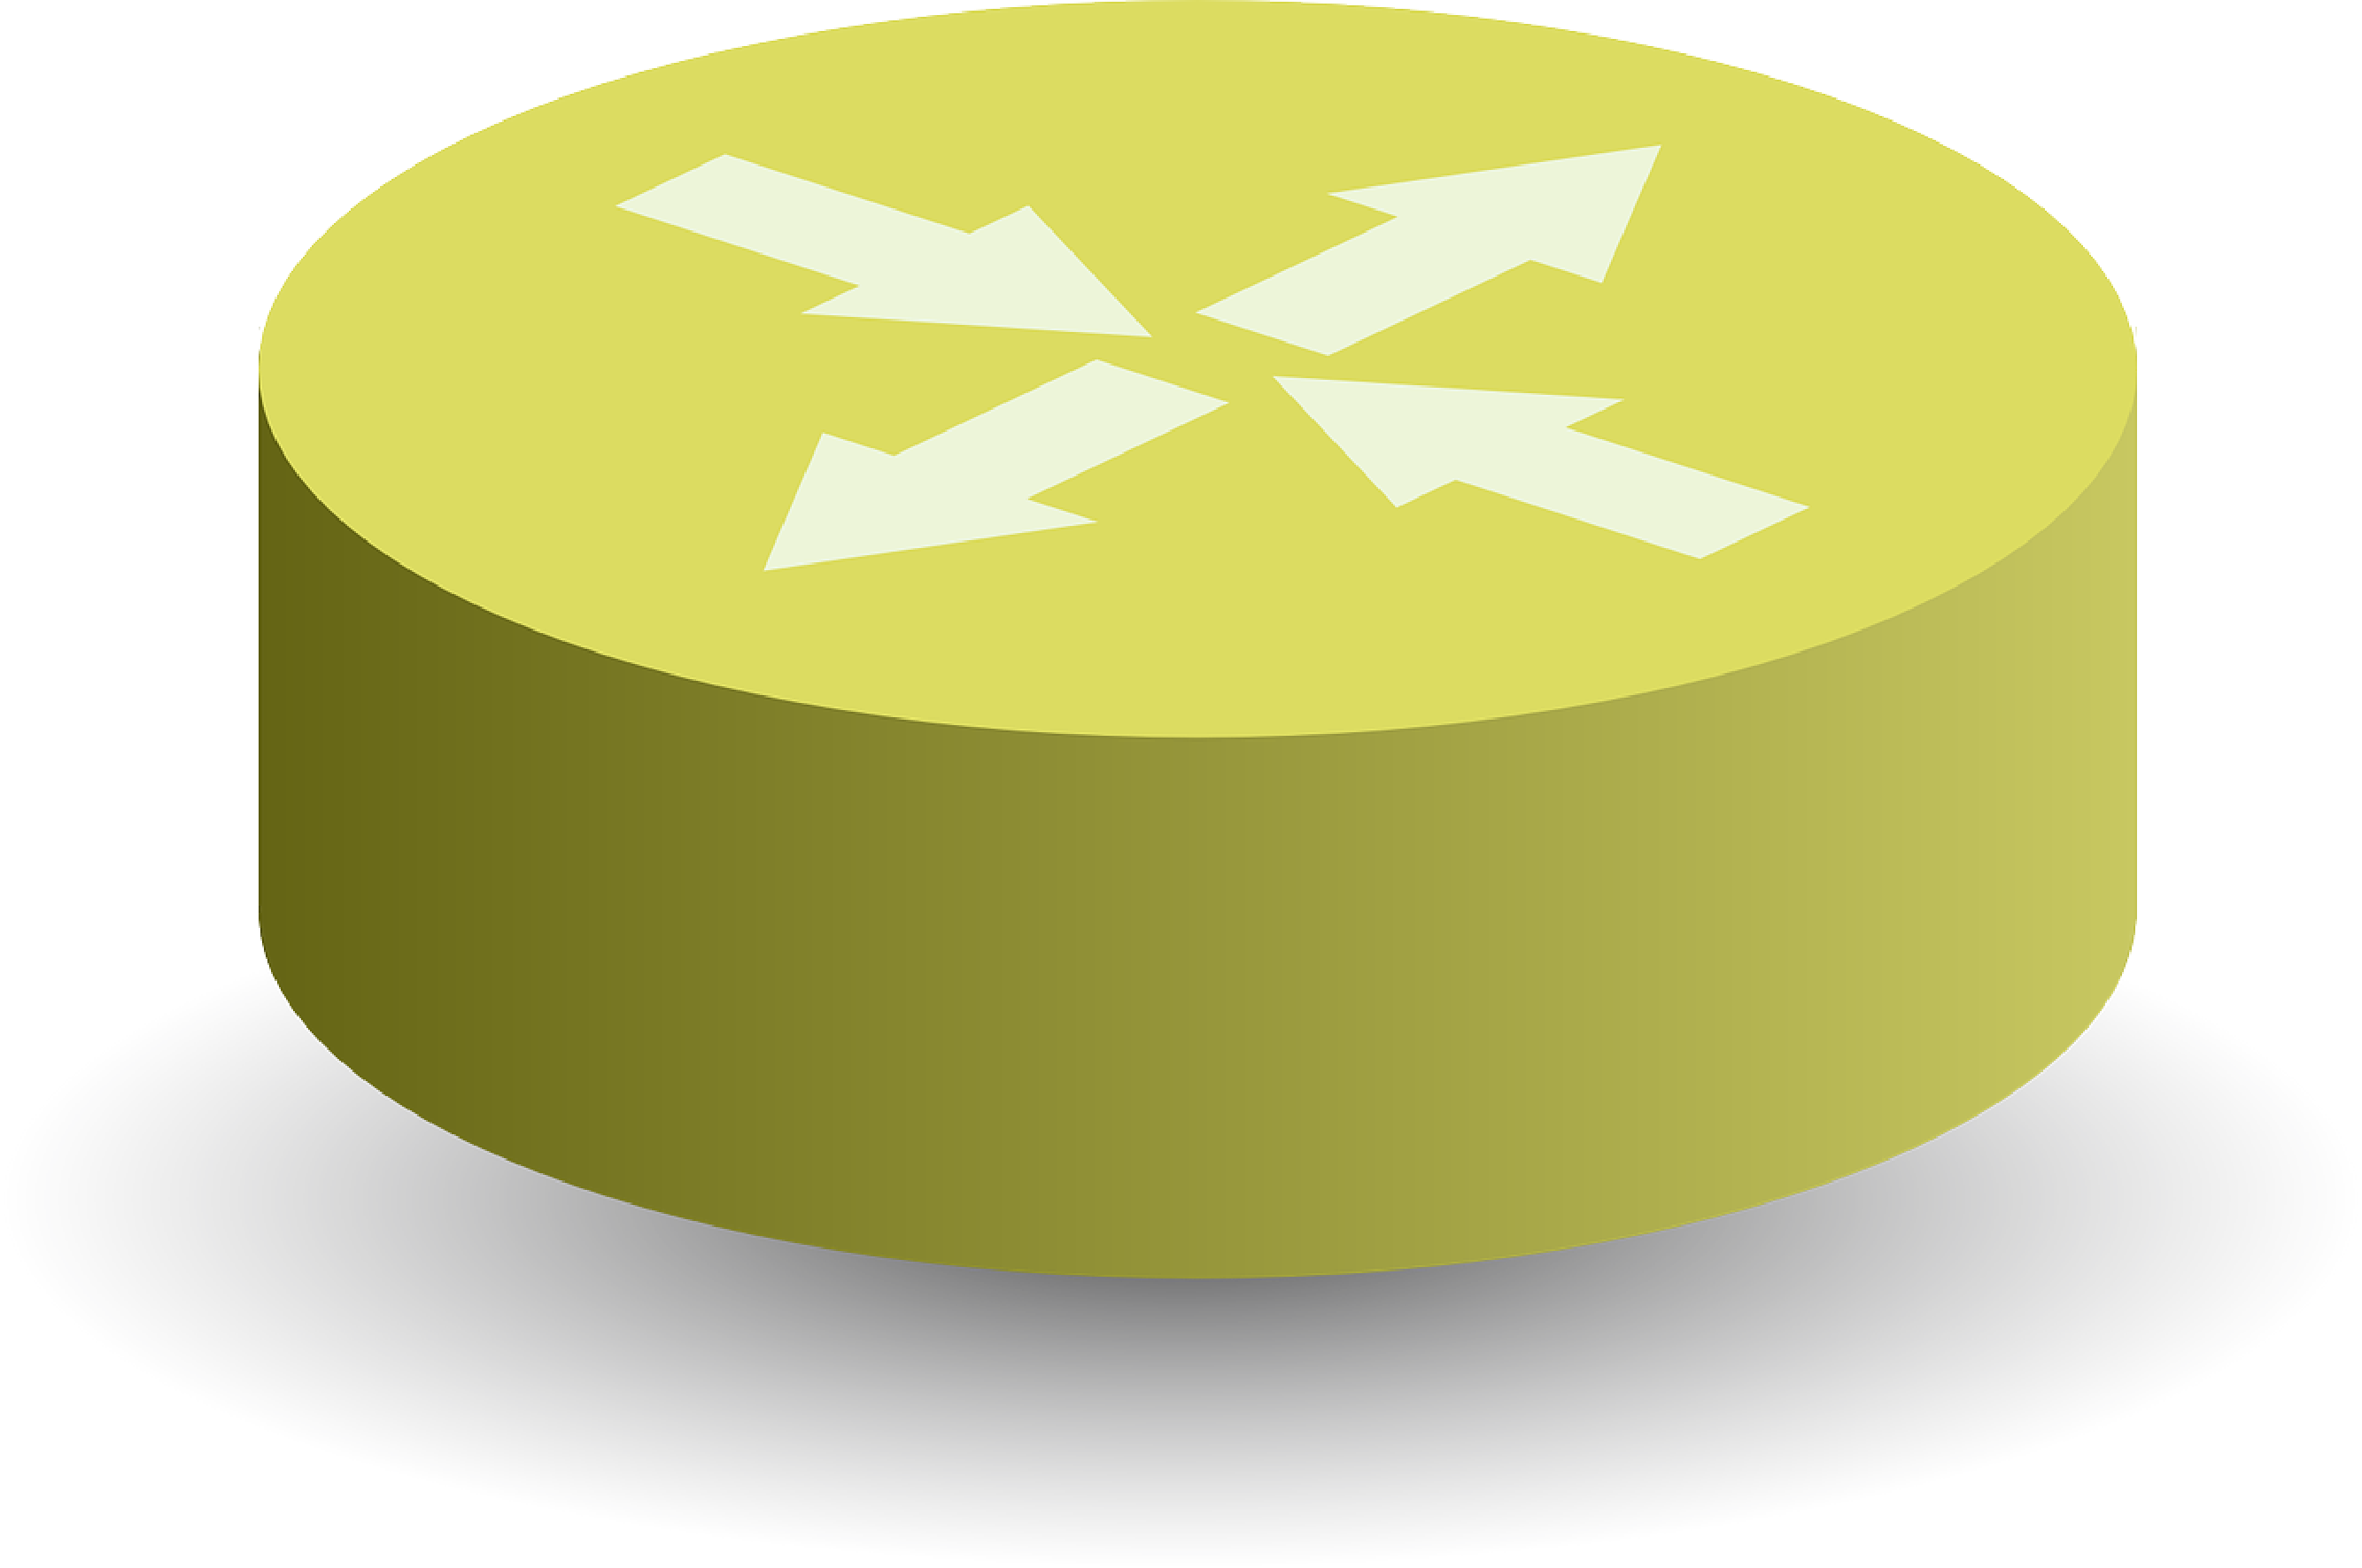
\includegraphics[width=52.5pt,height=52.5pt]{figures/router-158644_1280.pdf}};
%Image [id:dp04055959421826061] 
\draw (394.5,147.5) node  {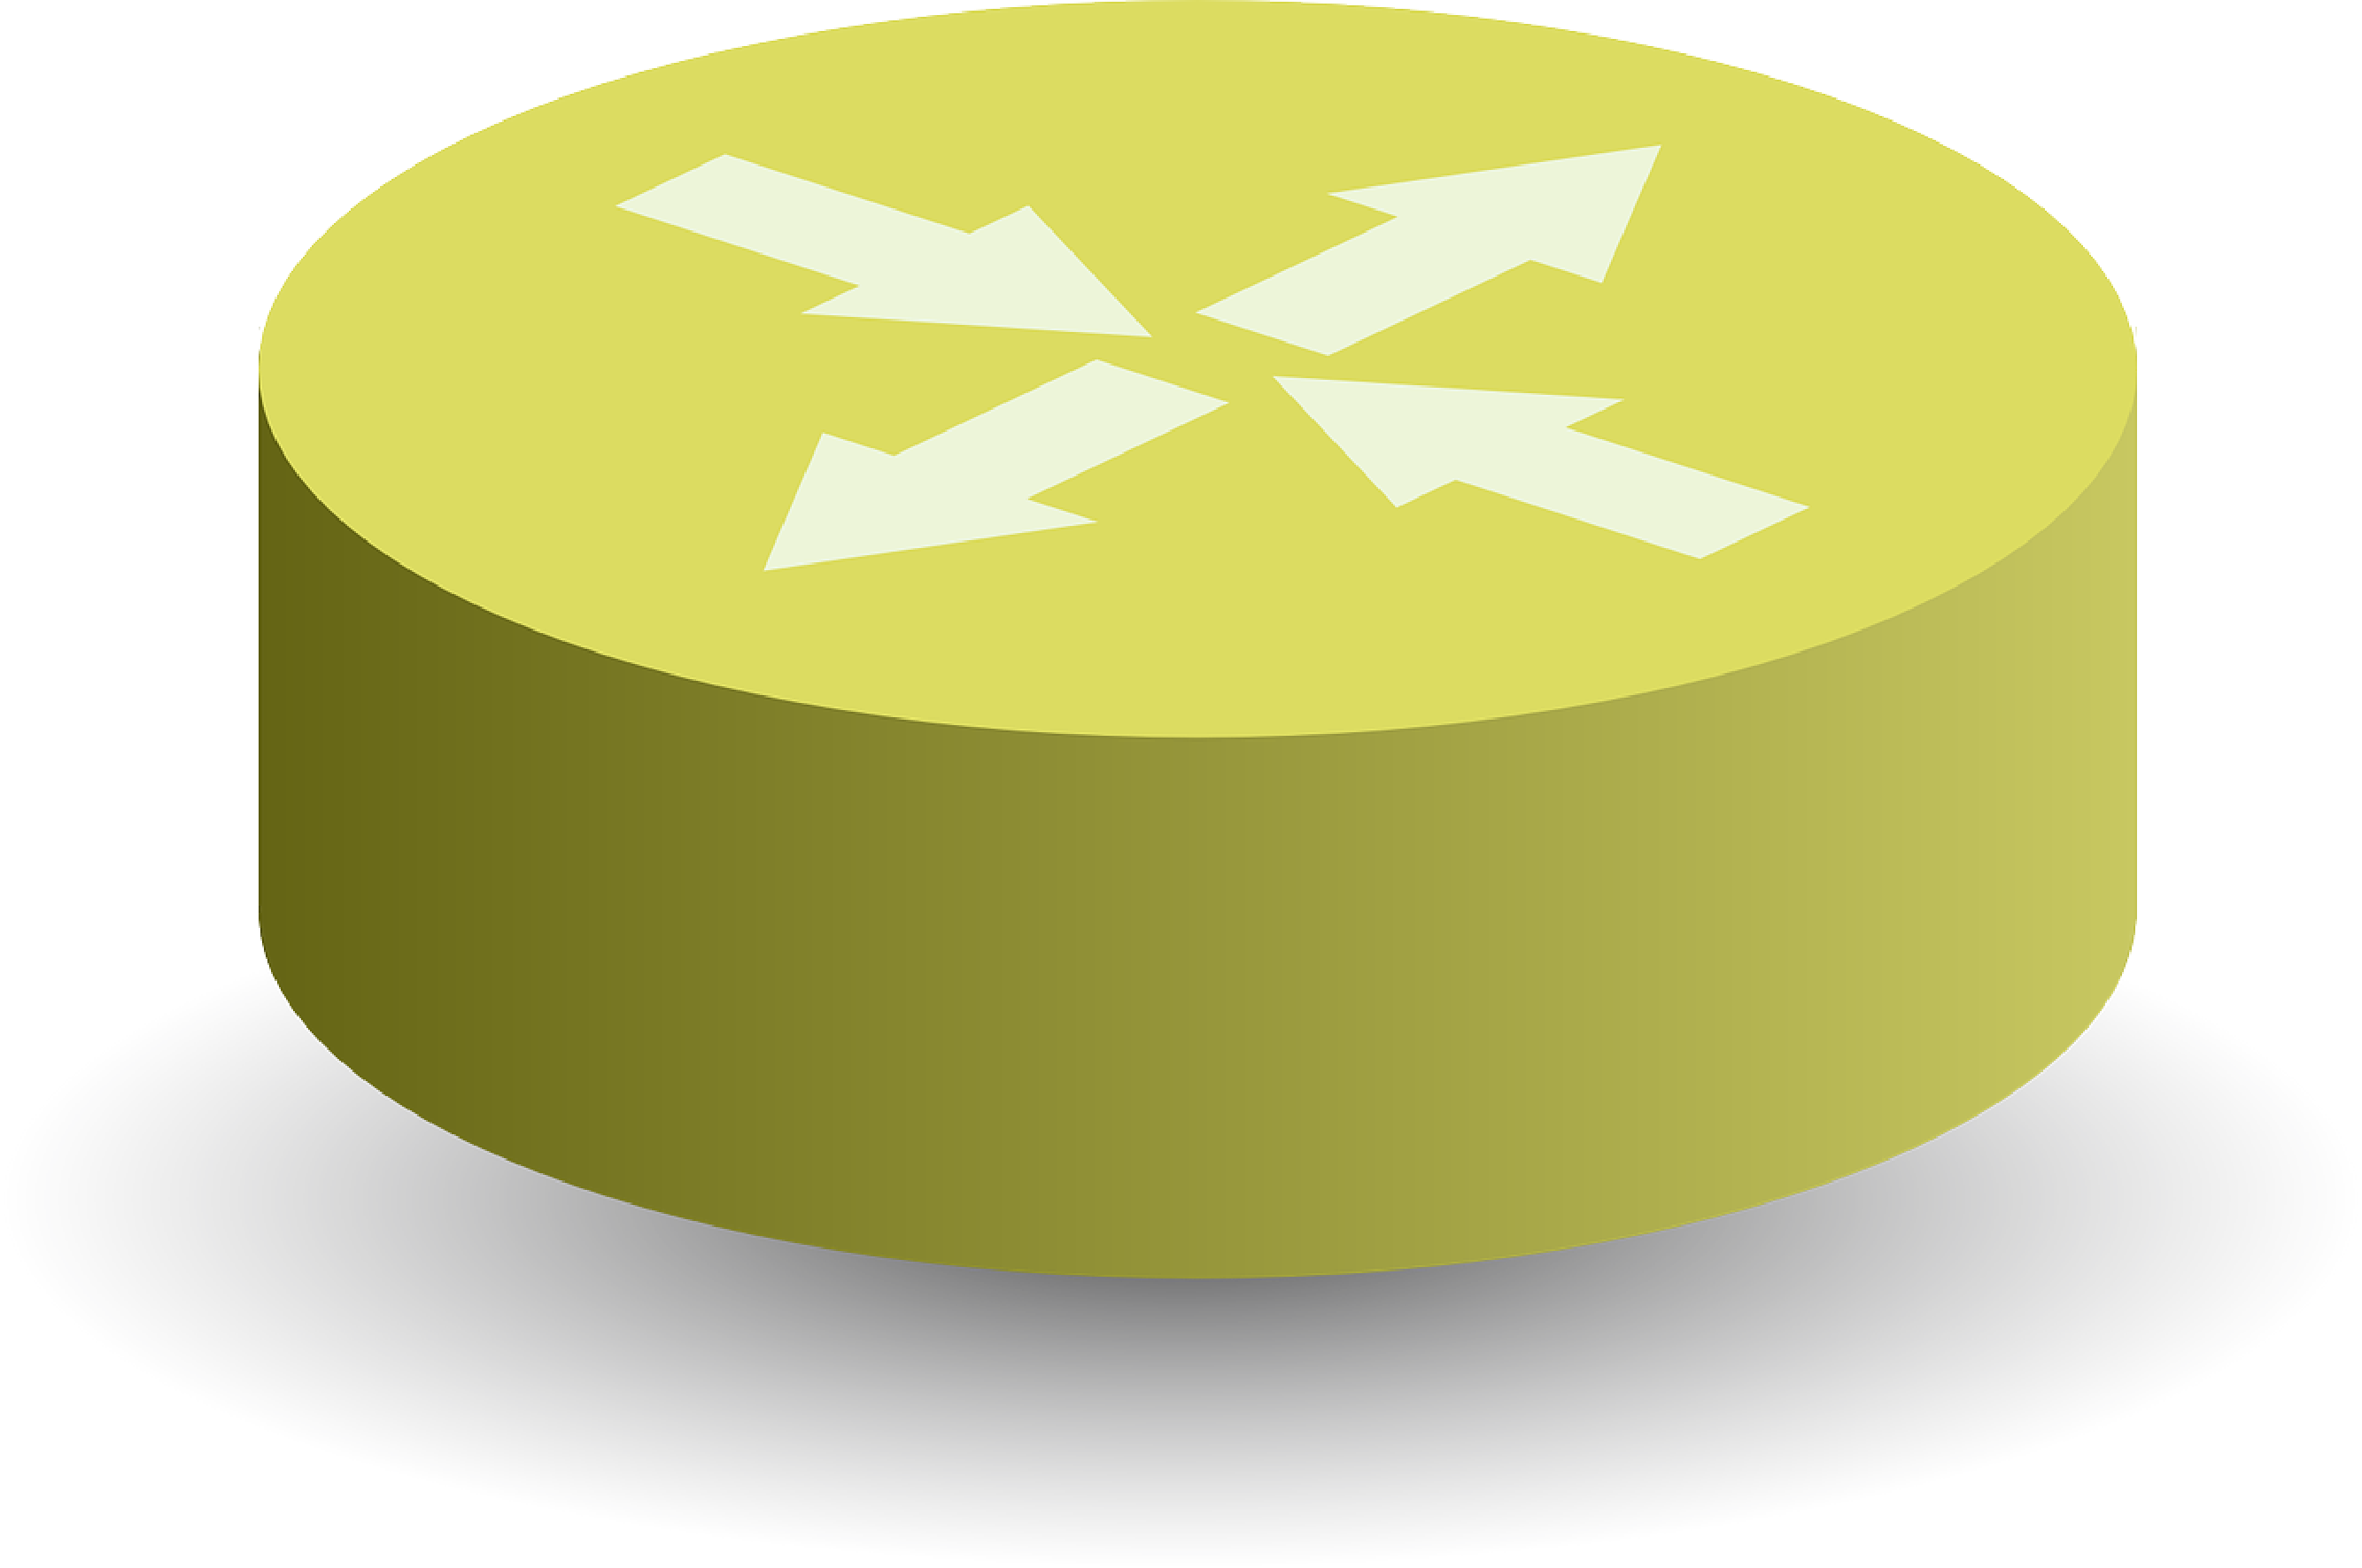
\includegraphics[width=52.5pt,height=52.5pt]{figures/router-158644_1280.pdf}};
%Image [id:dp9259427266230486] 
\draw (484,147.5) node  {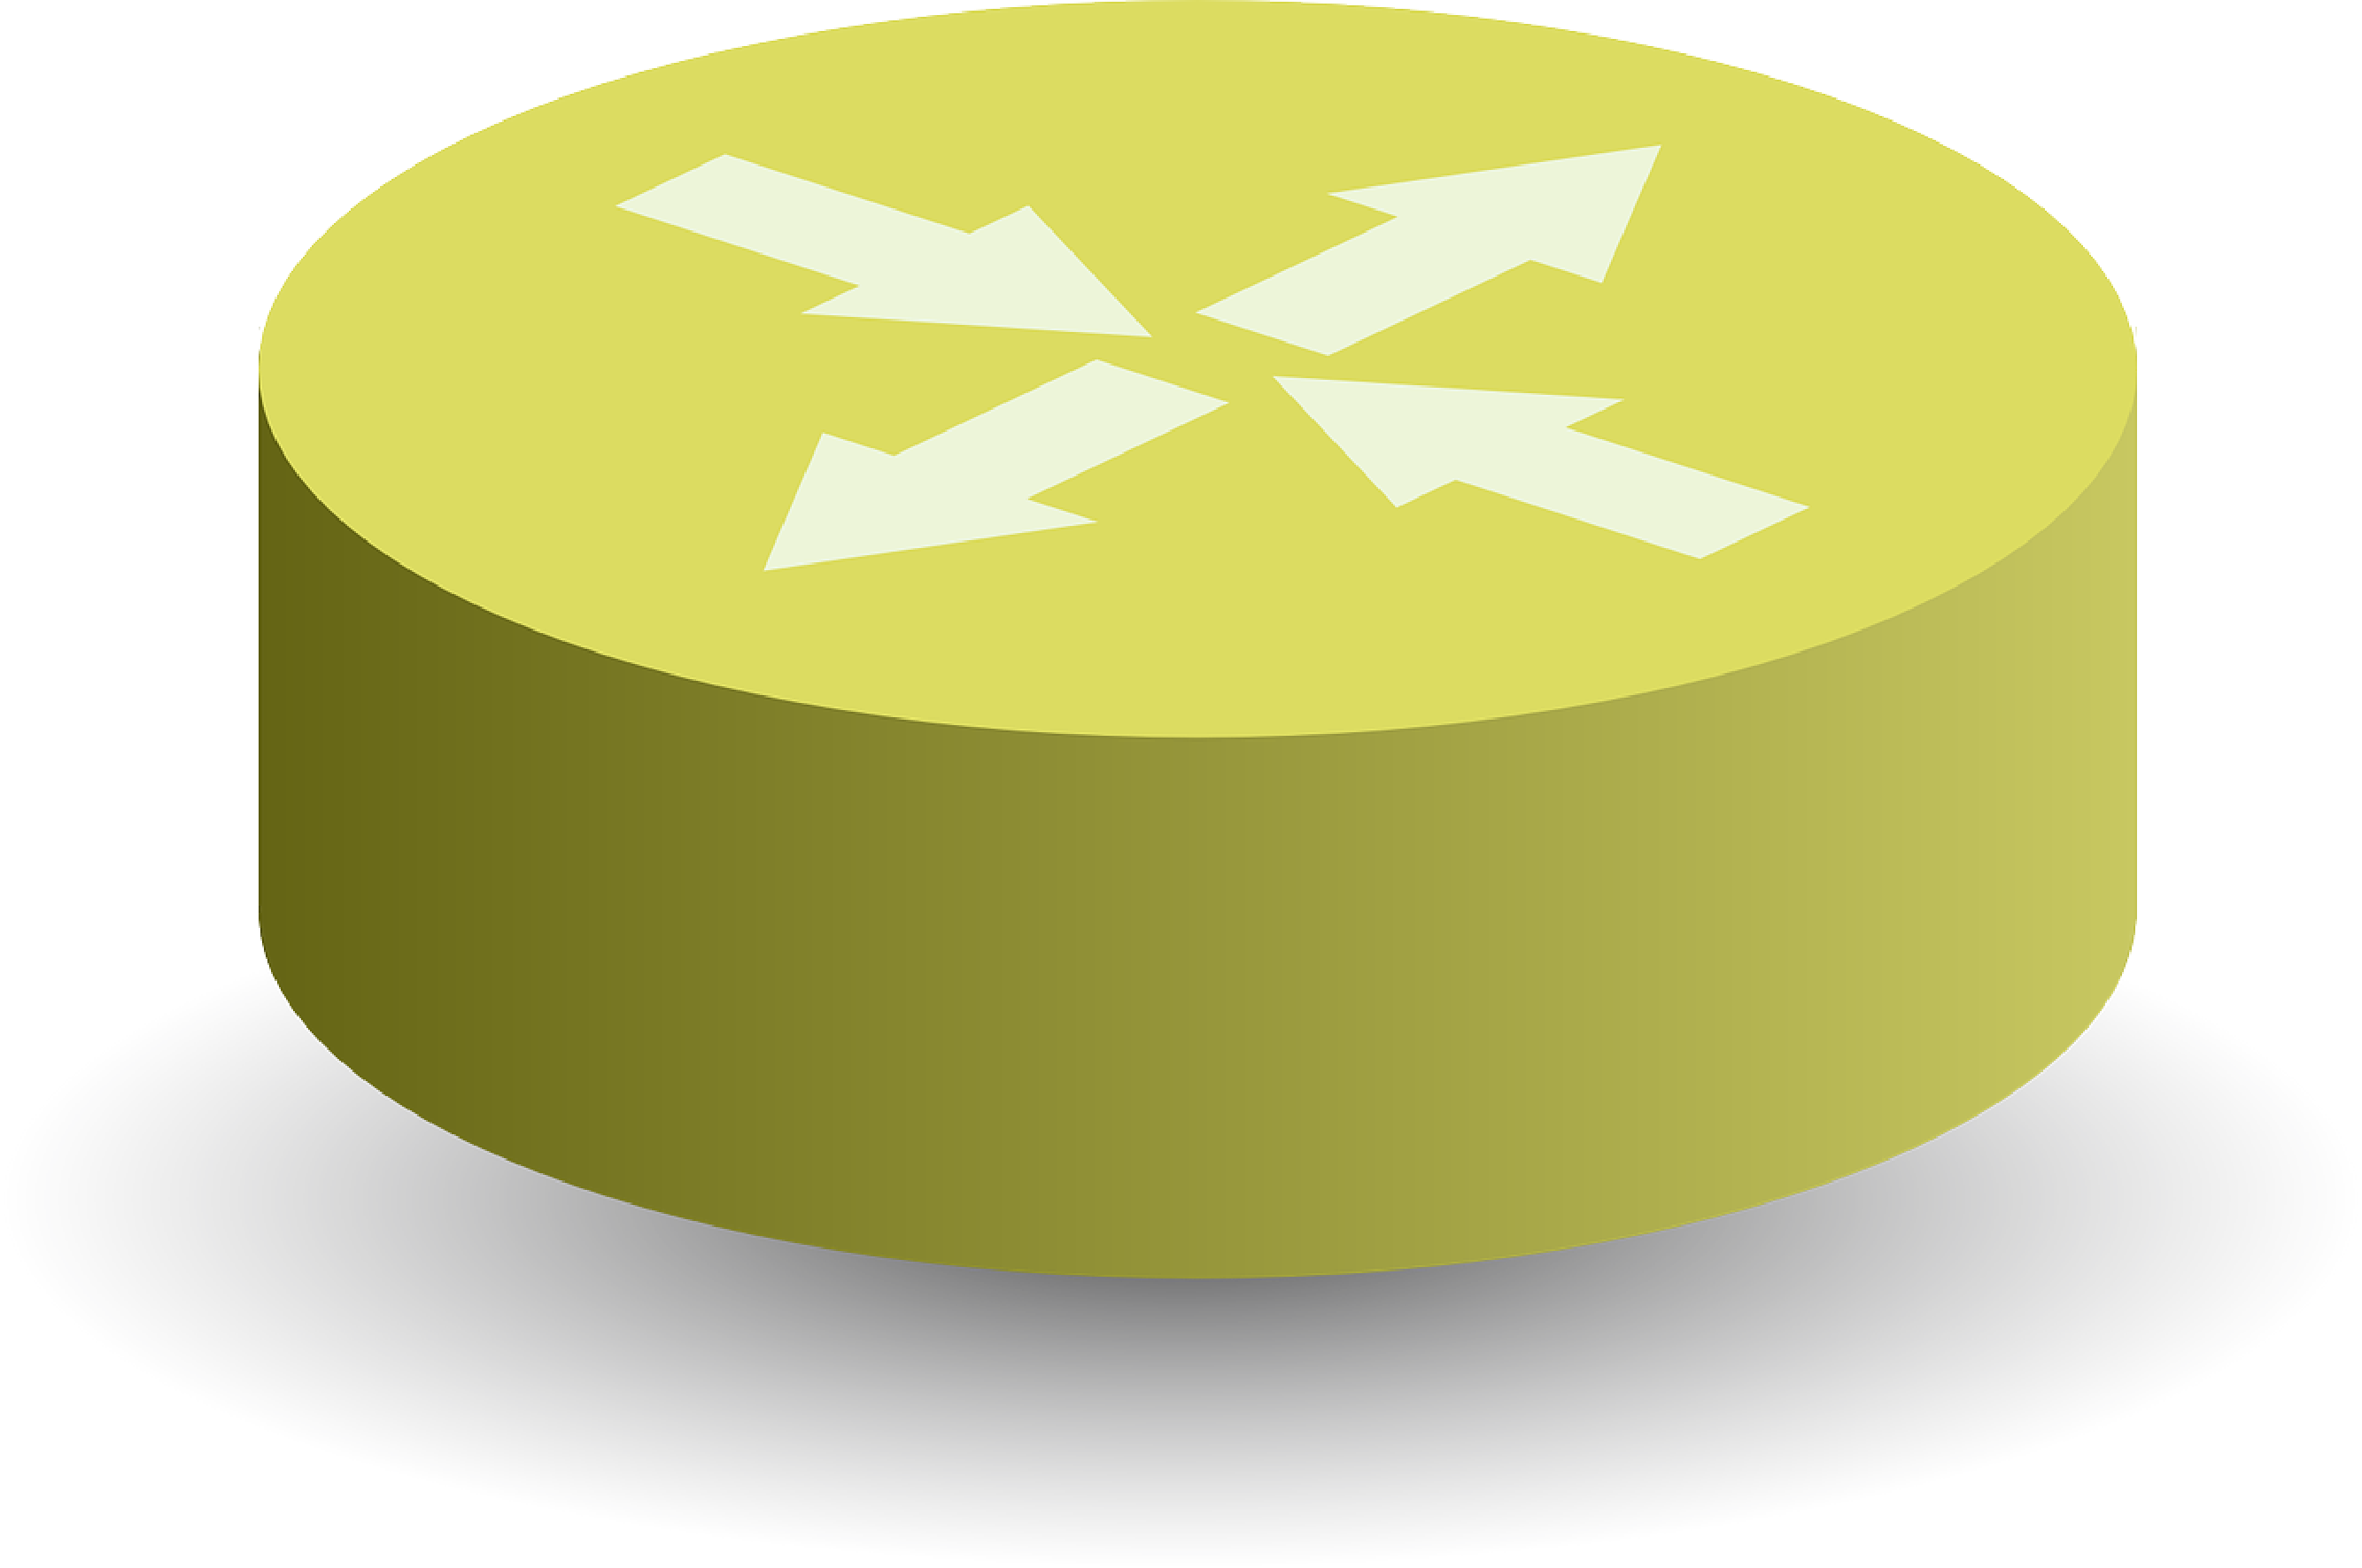
\includegraphics[width=52.5pt,height=52.5pt]{figures/router-158644_1280.pdf}};

%Rounded Rect [id:dp4478547267123999] 
\draw  [fill={rgb, 255:red, 255; green, 248; blue, 177 }  ,fill opacity=1 ] (26,125.27) .. controls (26,105.05) and (42.39,88.67) .. (62.6,88.67) -- (178.4,88.67) .. controls (198.61,88.67) and (215,105.05) .. (215,125.27) -- (215,235.07) .. controls (215,255.28) and (198.61,271.67) .. (178.4,271.67) -- (62.6,271.67) .. controls (42.39,271.67) and (26,255.28) .. (26,235.07) -- cycle ;
%Straight Lines [id:da04812807065340363] 
\draw    (56,180.67) -- (166,134.67) ;


%Image [id:dp341968705695737] 
\draw (61,184.5) node  {
\includegraphics[width=52.5pt,height=52.5pt]{figures/router-29825_1280.pdf}};
%Image [id:dp7725023918834623] 
\draw (165,130.5) node  {
\includegraphics[width=52.5pt,height=52.5pt]{figures/router-29825_1280.pdf}};

%Straight Lines [id:da036026819015278266] 
\draw    (81,200.17) -- (138,225.67) ;


%Image [id:dp29149867233304716] 
\draw (136,238.5) node  {
\includegraphics[width=52.5pt,height=52.5pt]{figures/router-29825_1280.pdf}};

%Rounded Rect [id:dp8669891034149613] 
\draw  [fill={rgb, 255:red, 184; green, 233; blue, 134 }  ,fill opacity=1 ] (8,398.47) .. controls (8,383.11) and (20.45,370.67) .. (35.8,370.67) -- (583.2,370.67) .. controls (598.55,370.67) and (611,383.11) .. (611,398.47) -- (611,481.87) .. controls (611,497.22) and (598.55,509.67) .. (583.2,509.67) -- (35.8,509.67) .. controls (20.45,509.67) and (8,497.22) .. (8,481.87) -- cycle ;
%Straight Lines [id:da7257050611297167] 
\draw    (79,428.67) -- (214,401.67) ;


%Straight Lines [id:da6984840894149047] 
\draw    (80,443.67) -- (171,466.67) ;


%Straight Lines [id:da6802535311385733] 
\draw    (174,473.67) -- (368,426.67) ;


%Straight Lines [id:da14214857377238777] 
\draw    (214,401.67) -- (358,410.67) ;


%Straight Lines [id:da6556428261701027] 
\draw    (384,420.67) -- (502,407.67) ;


%Straight Lines [id:da16066583484396146] 
\draw    (375,440.67) -- (477,476.67) ;


%Image [id:dp1703433460369157] 
\draw (70,443.5) node  {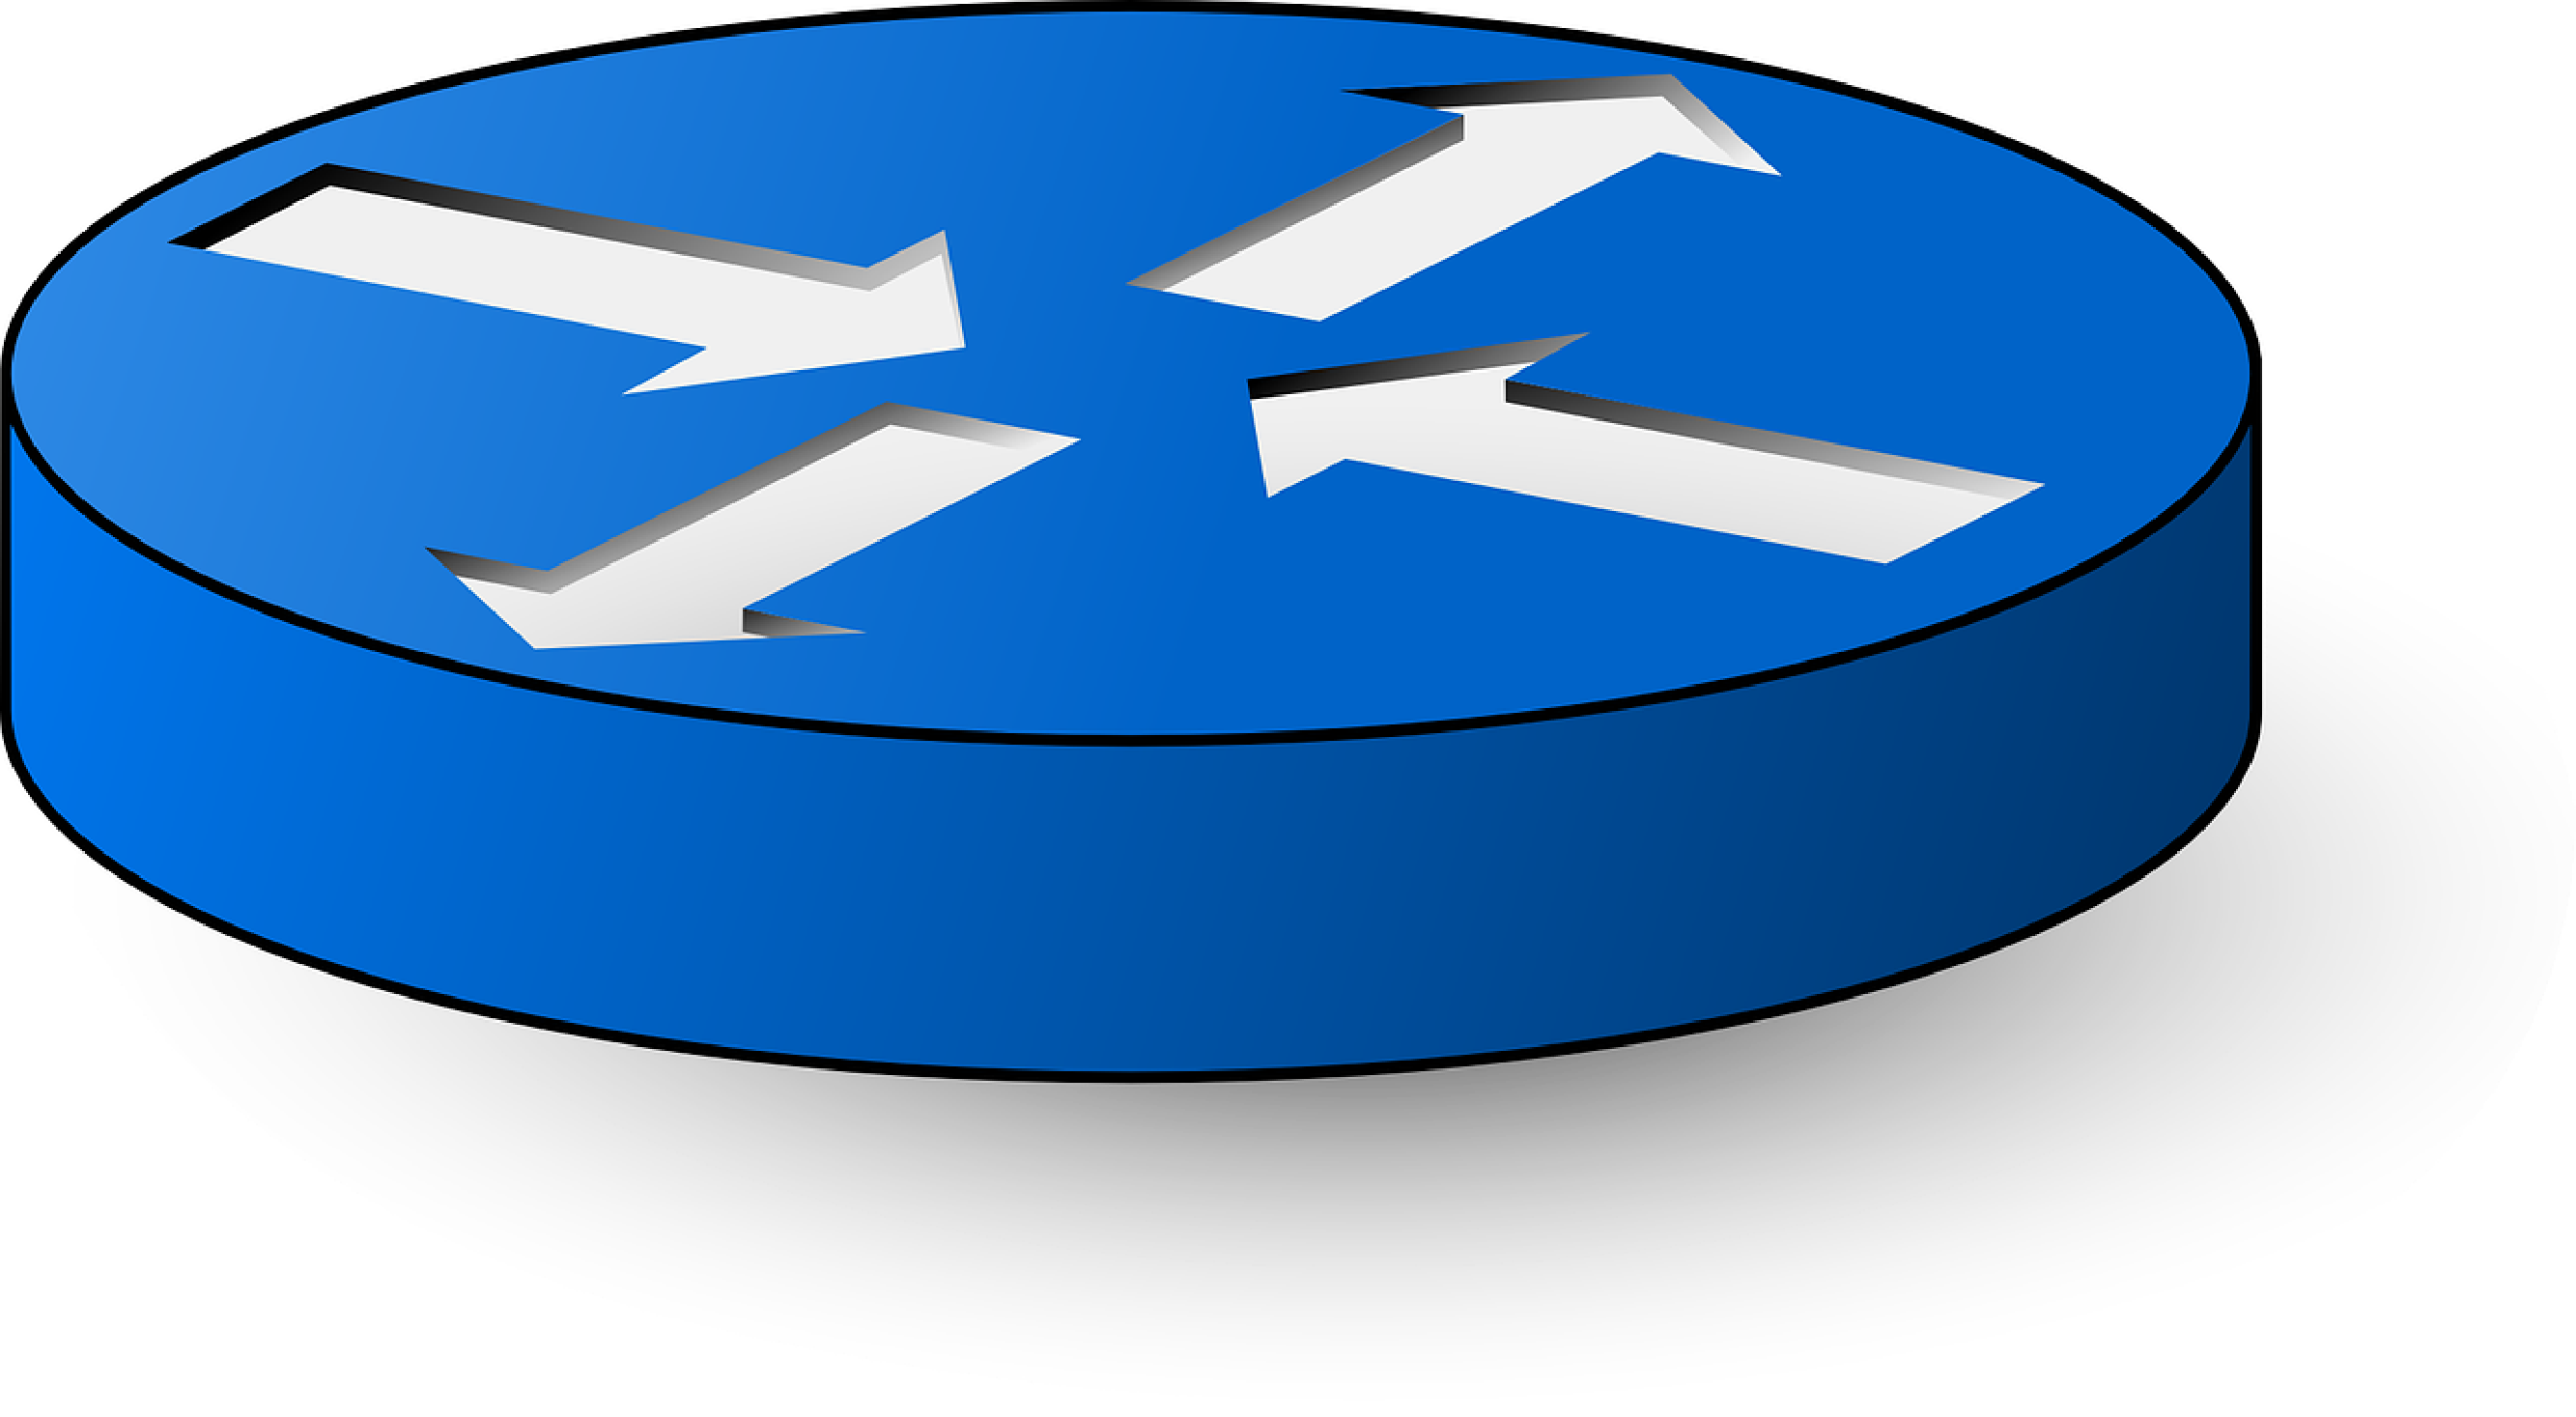
\includegraphics[width=52.5pt,height=52.5pt]{figures/router-30140_1280.pdf}};
%Image [id:dp7119657242561229] 
\draw (160,474.5) node  {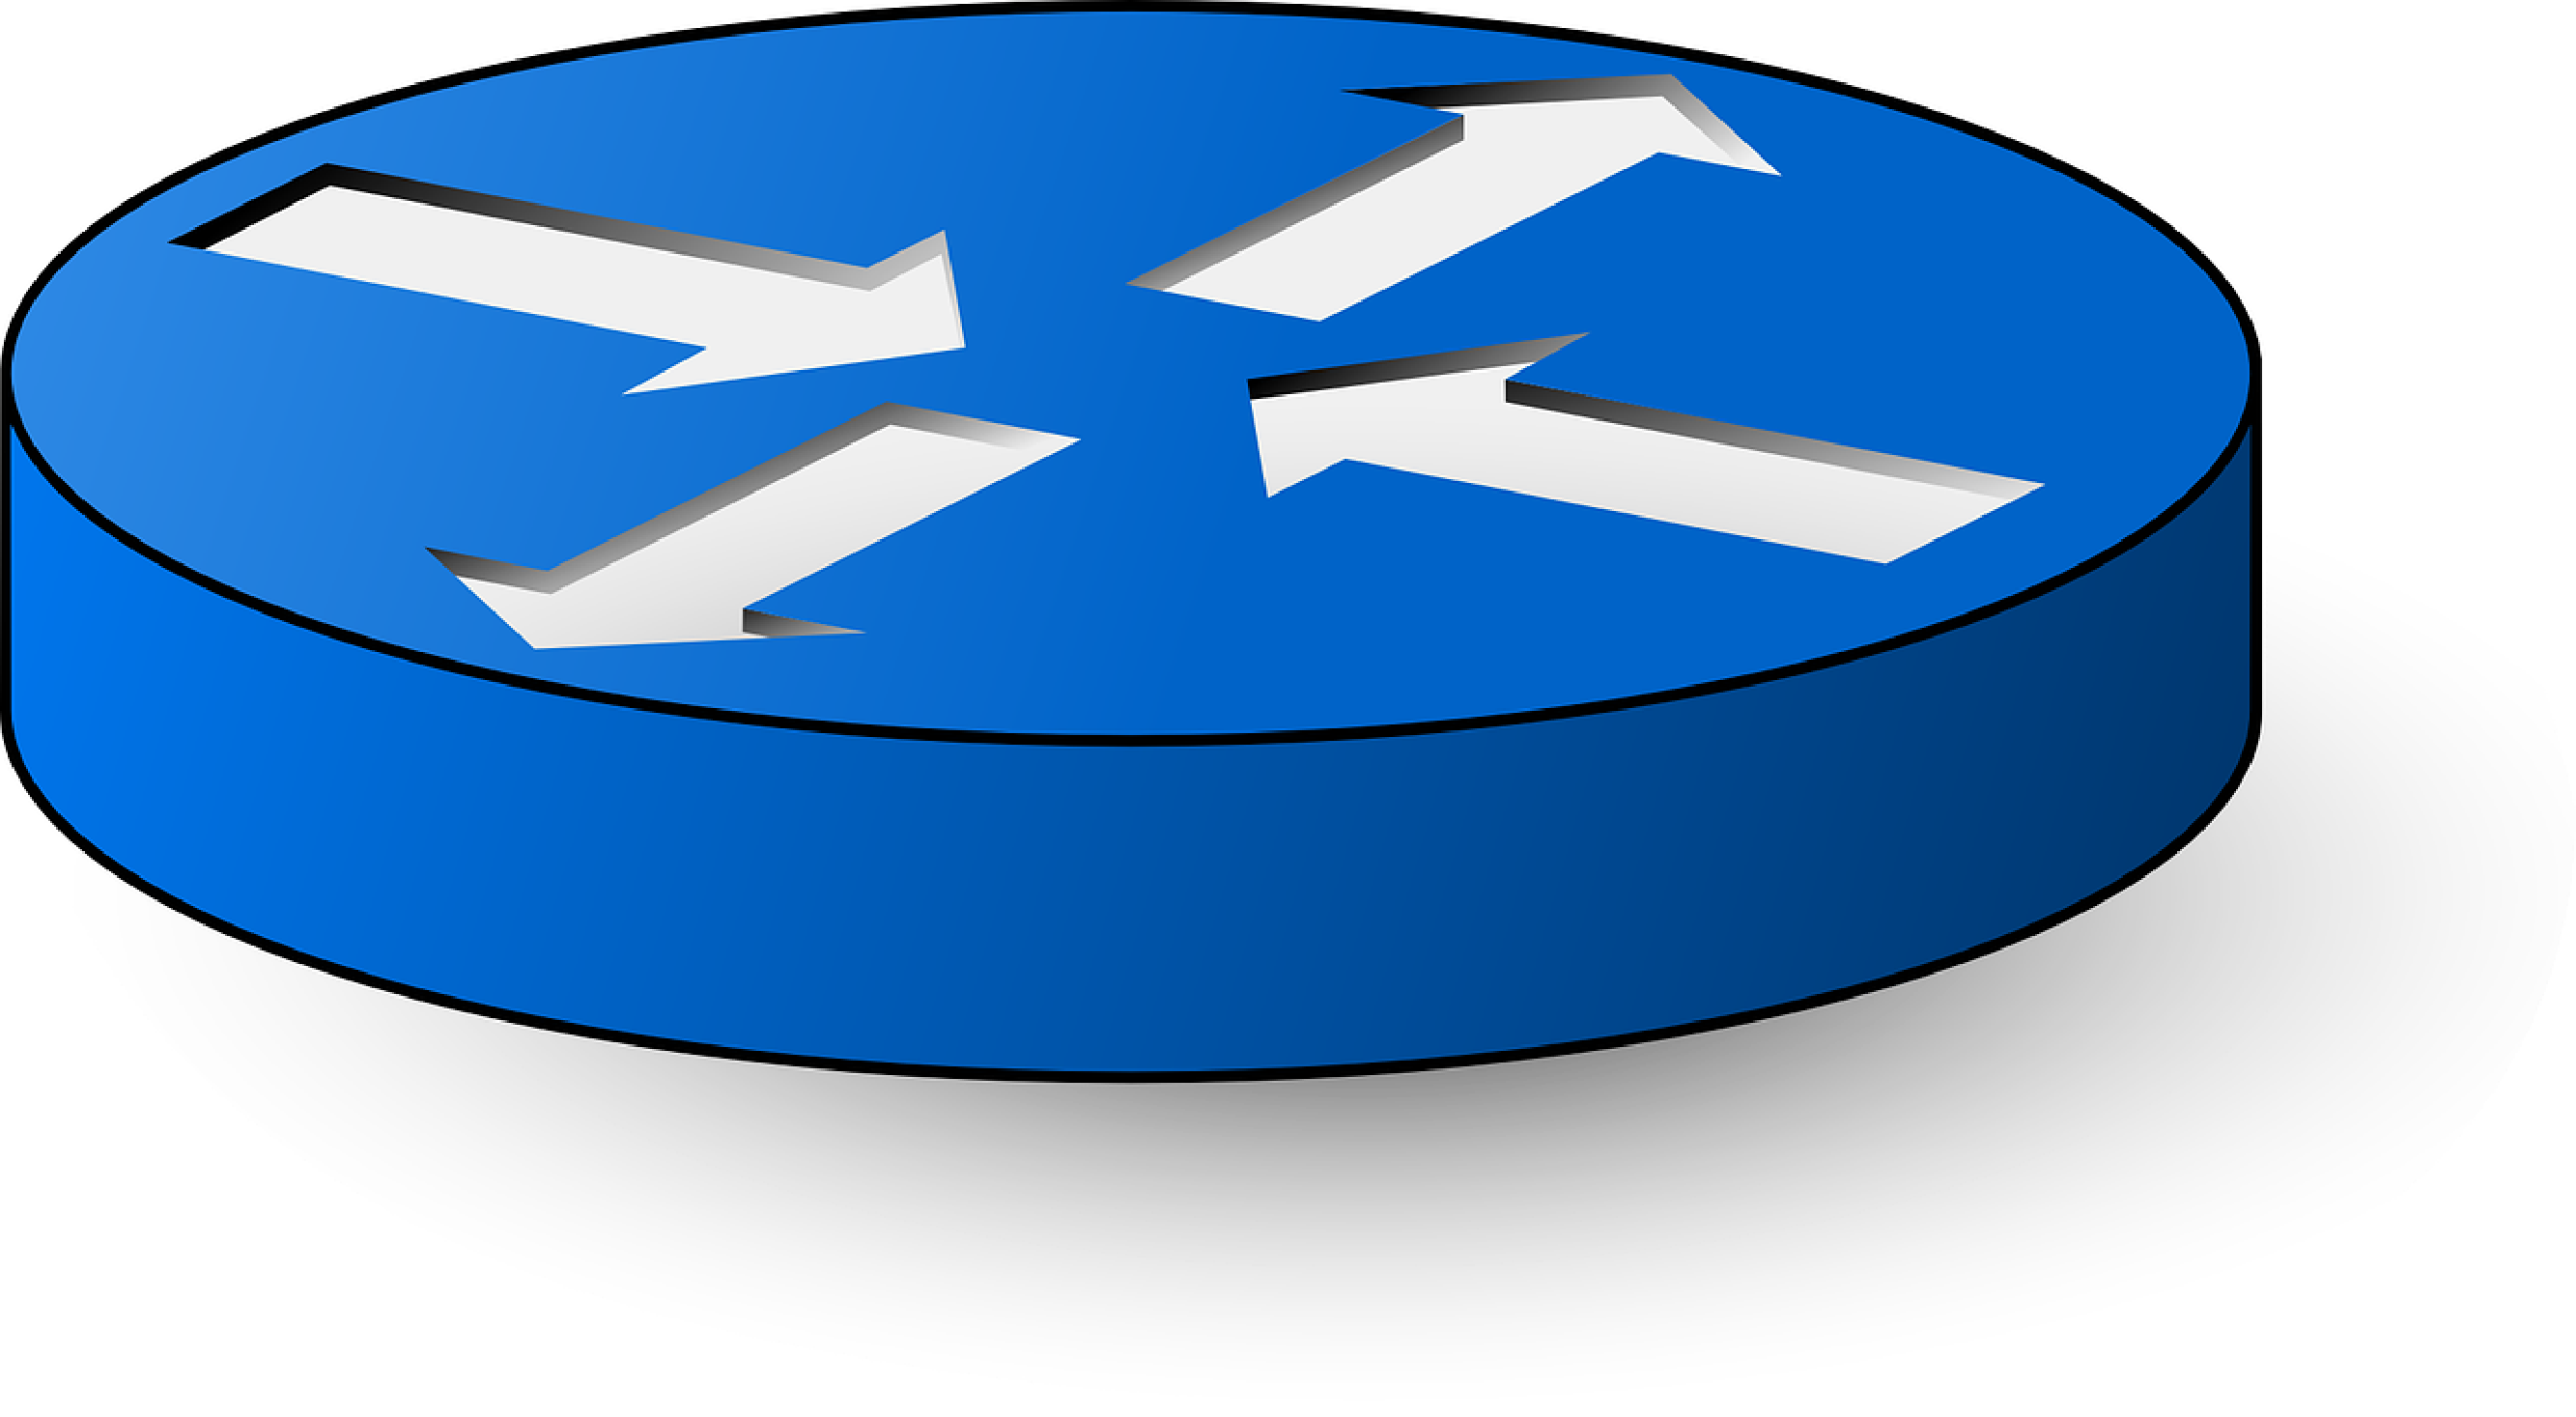
\includegraphics[width=52.5pt,height=52.5pt]{figures/router-30140_1280.pdf}};
%Image [id:dp01793726972424281] 
\draw (200,411.5) node  {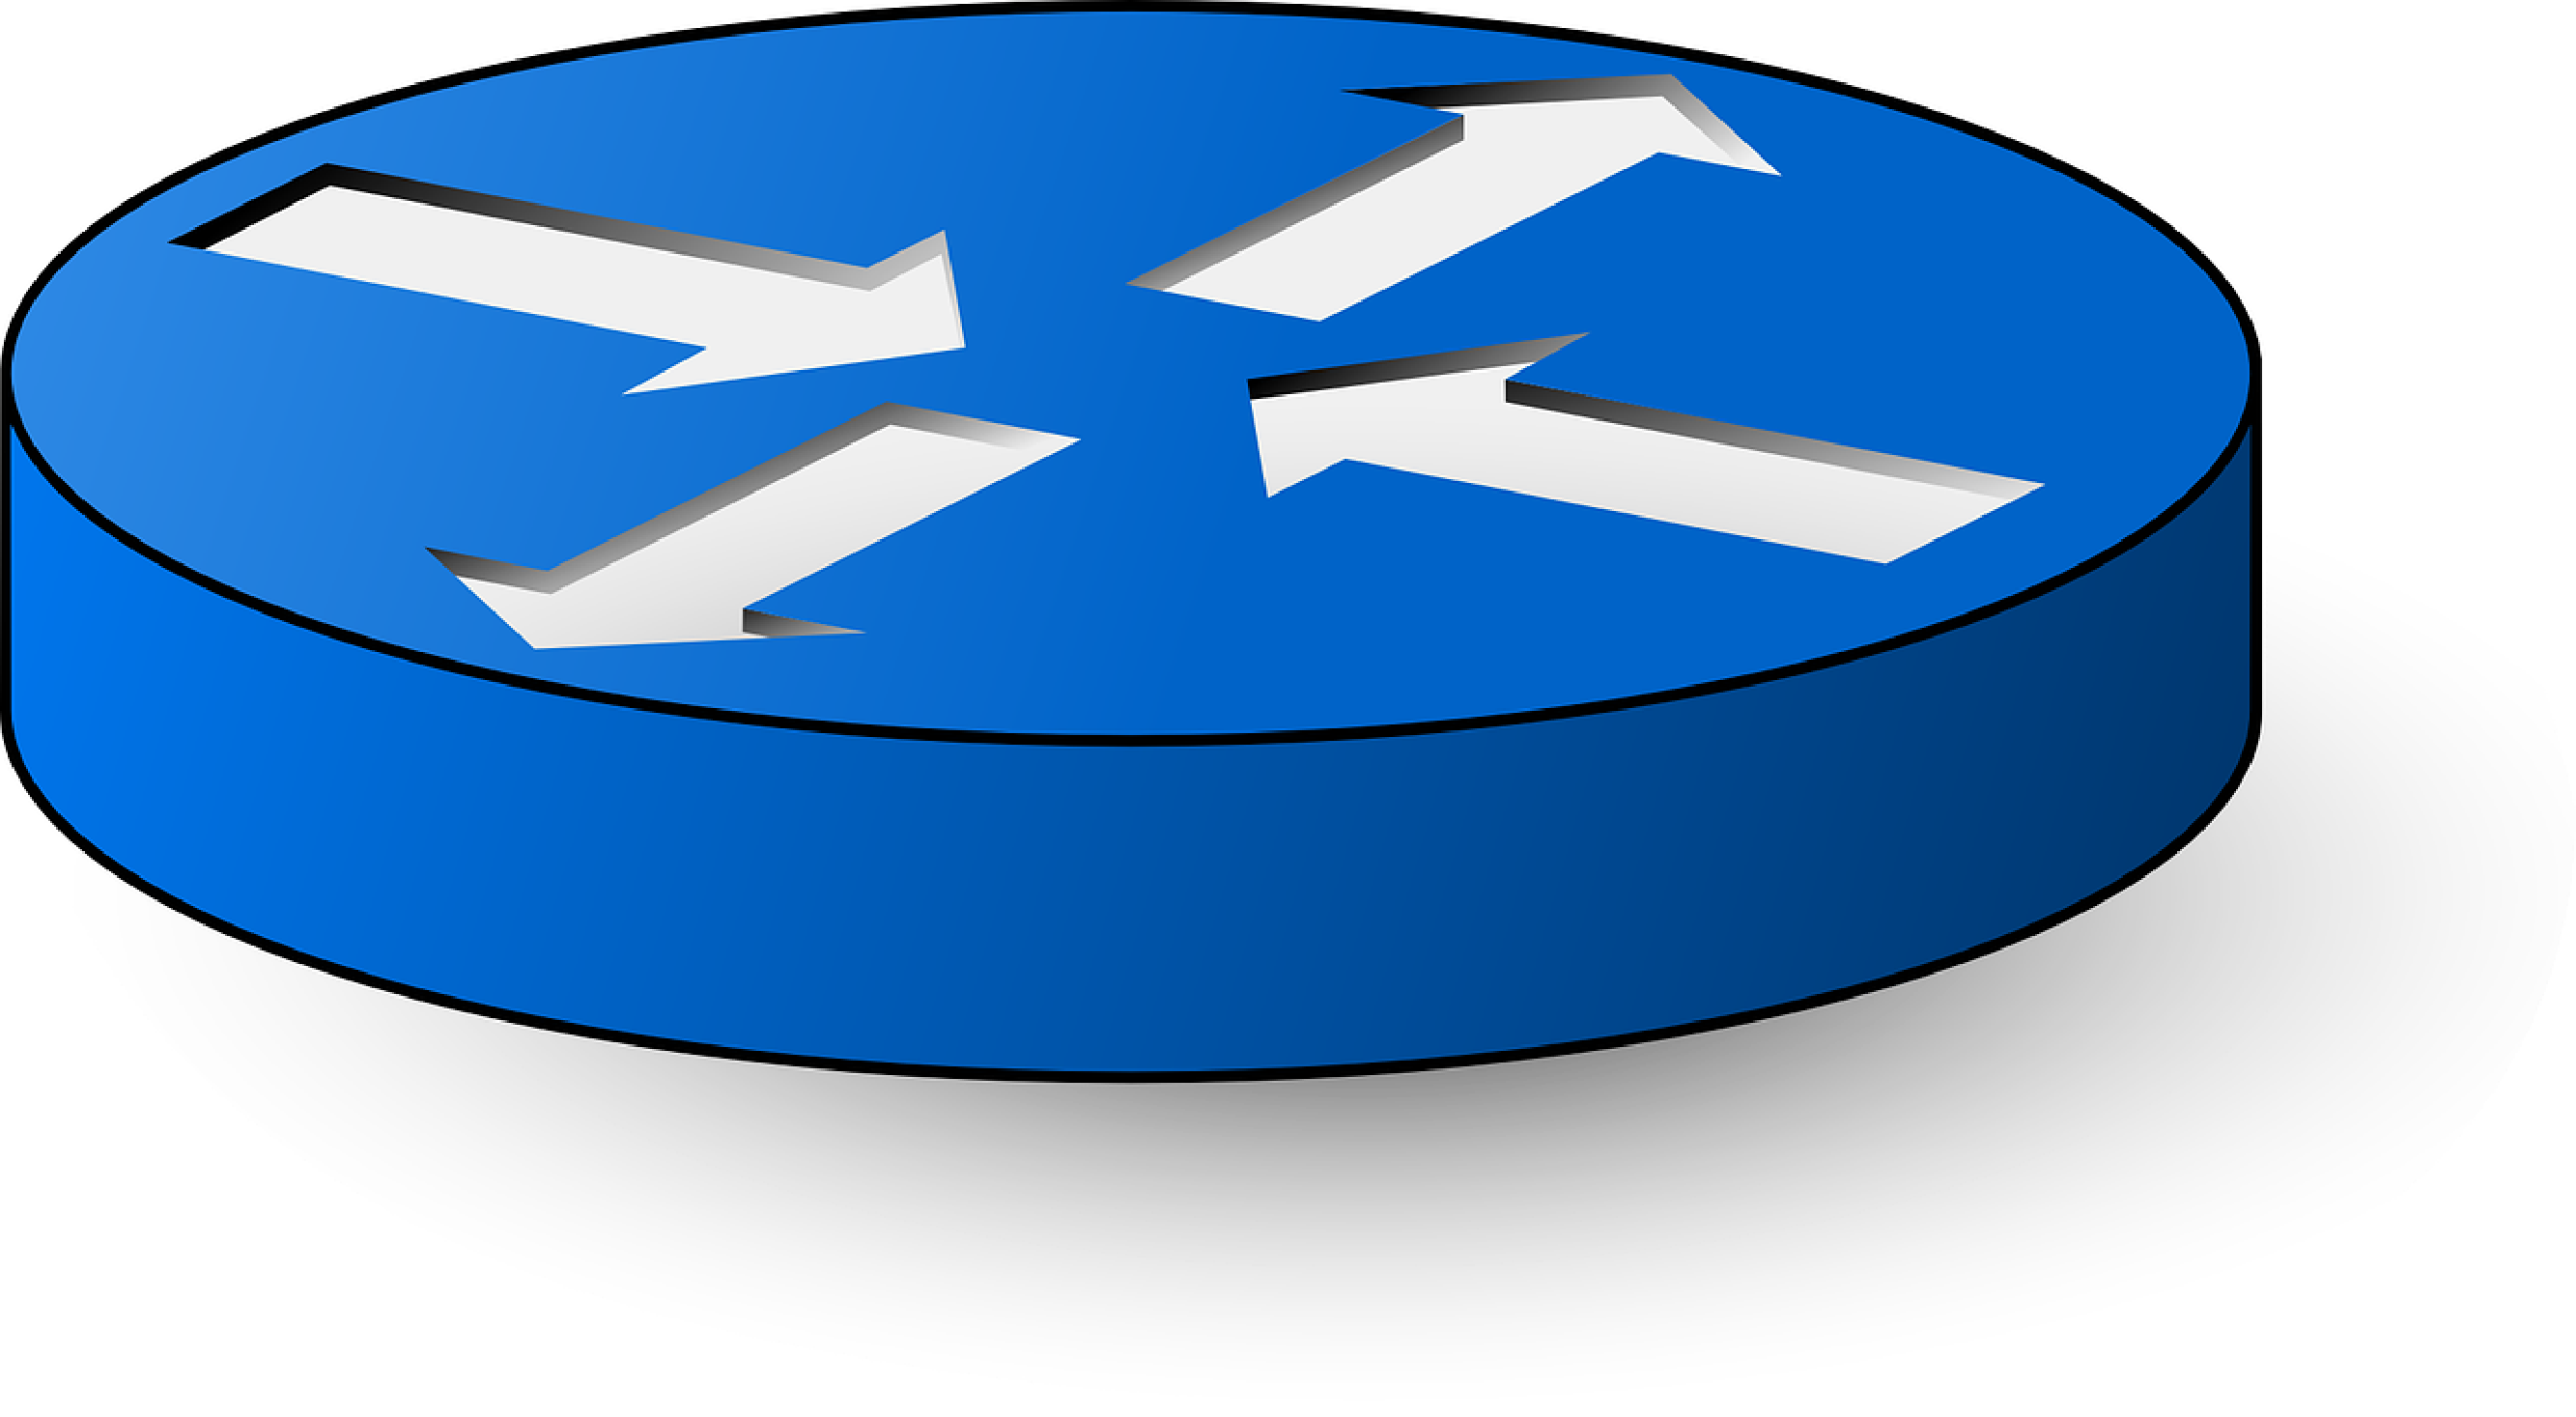
\includegraphics[width=52.5pt,height=52.5pt]{figures/router-30140_1280.pdf}};
%Image [id:dp9361502418924952] 
\draw (386,425.5) node  {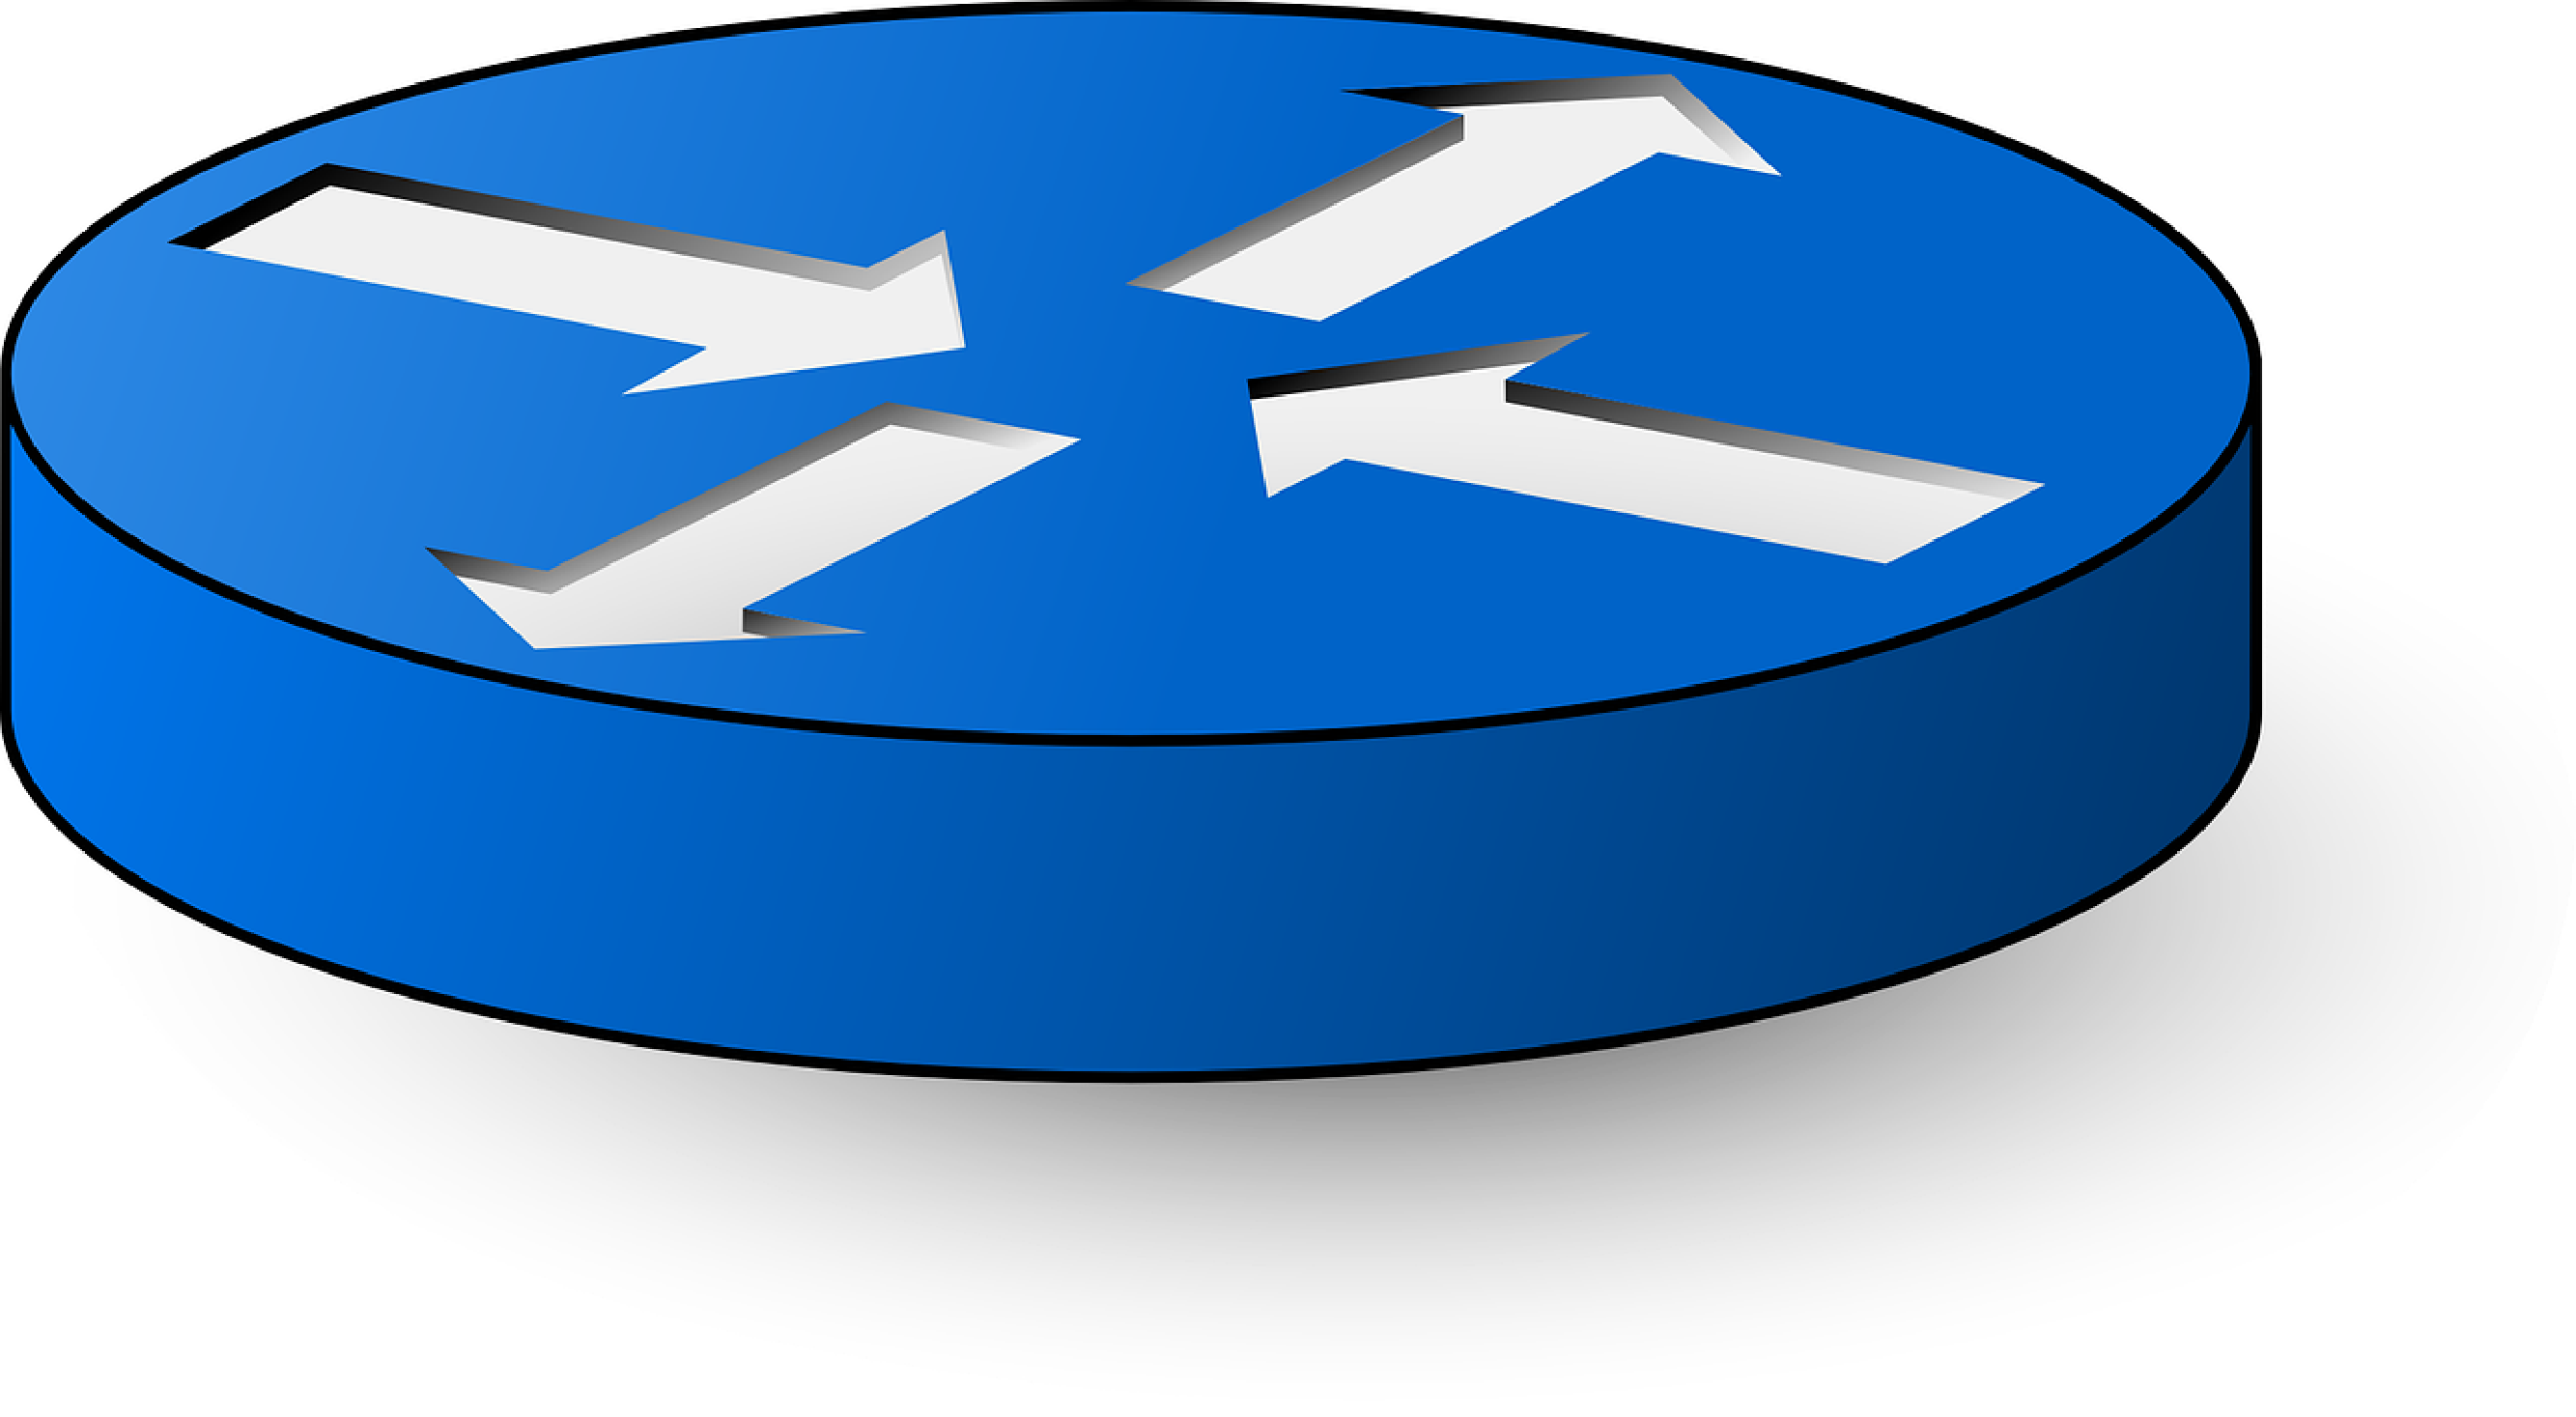
\includegraphics[width=52.5pt,height=52.5pt]{figures/router-30140_1280.pdf}};
%Image [id:dp1834582453825948] 
\draw (515,414.5) node  {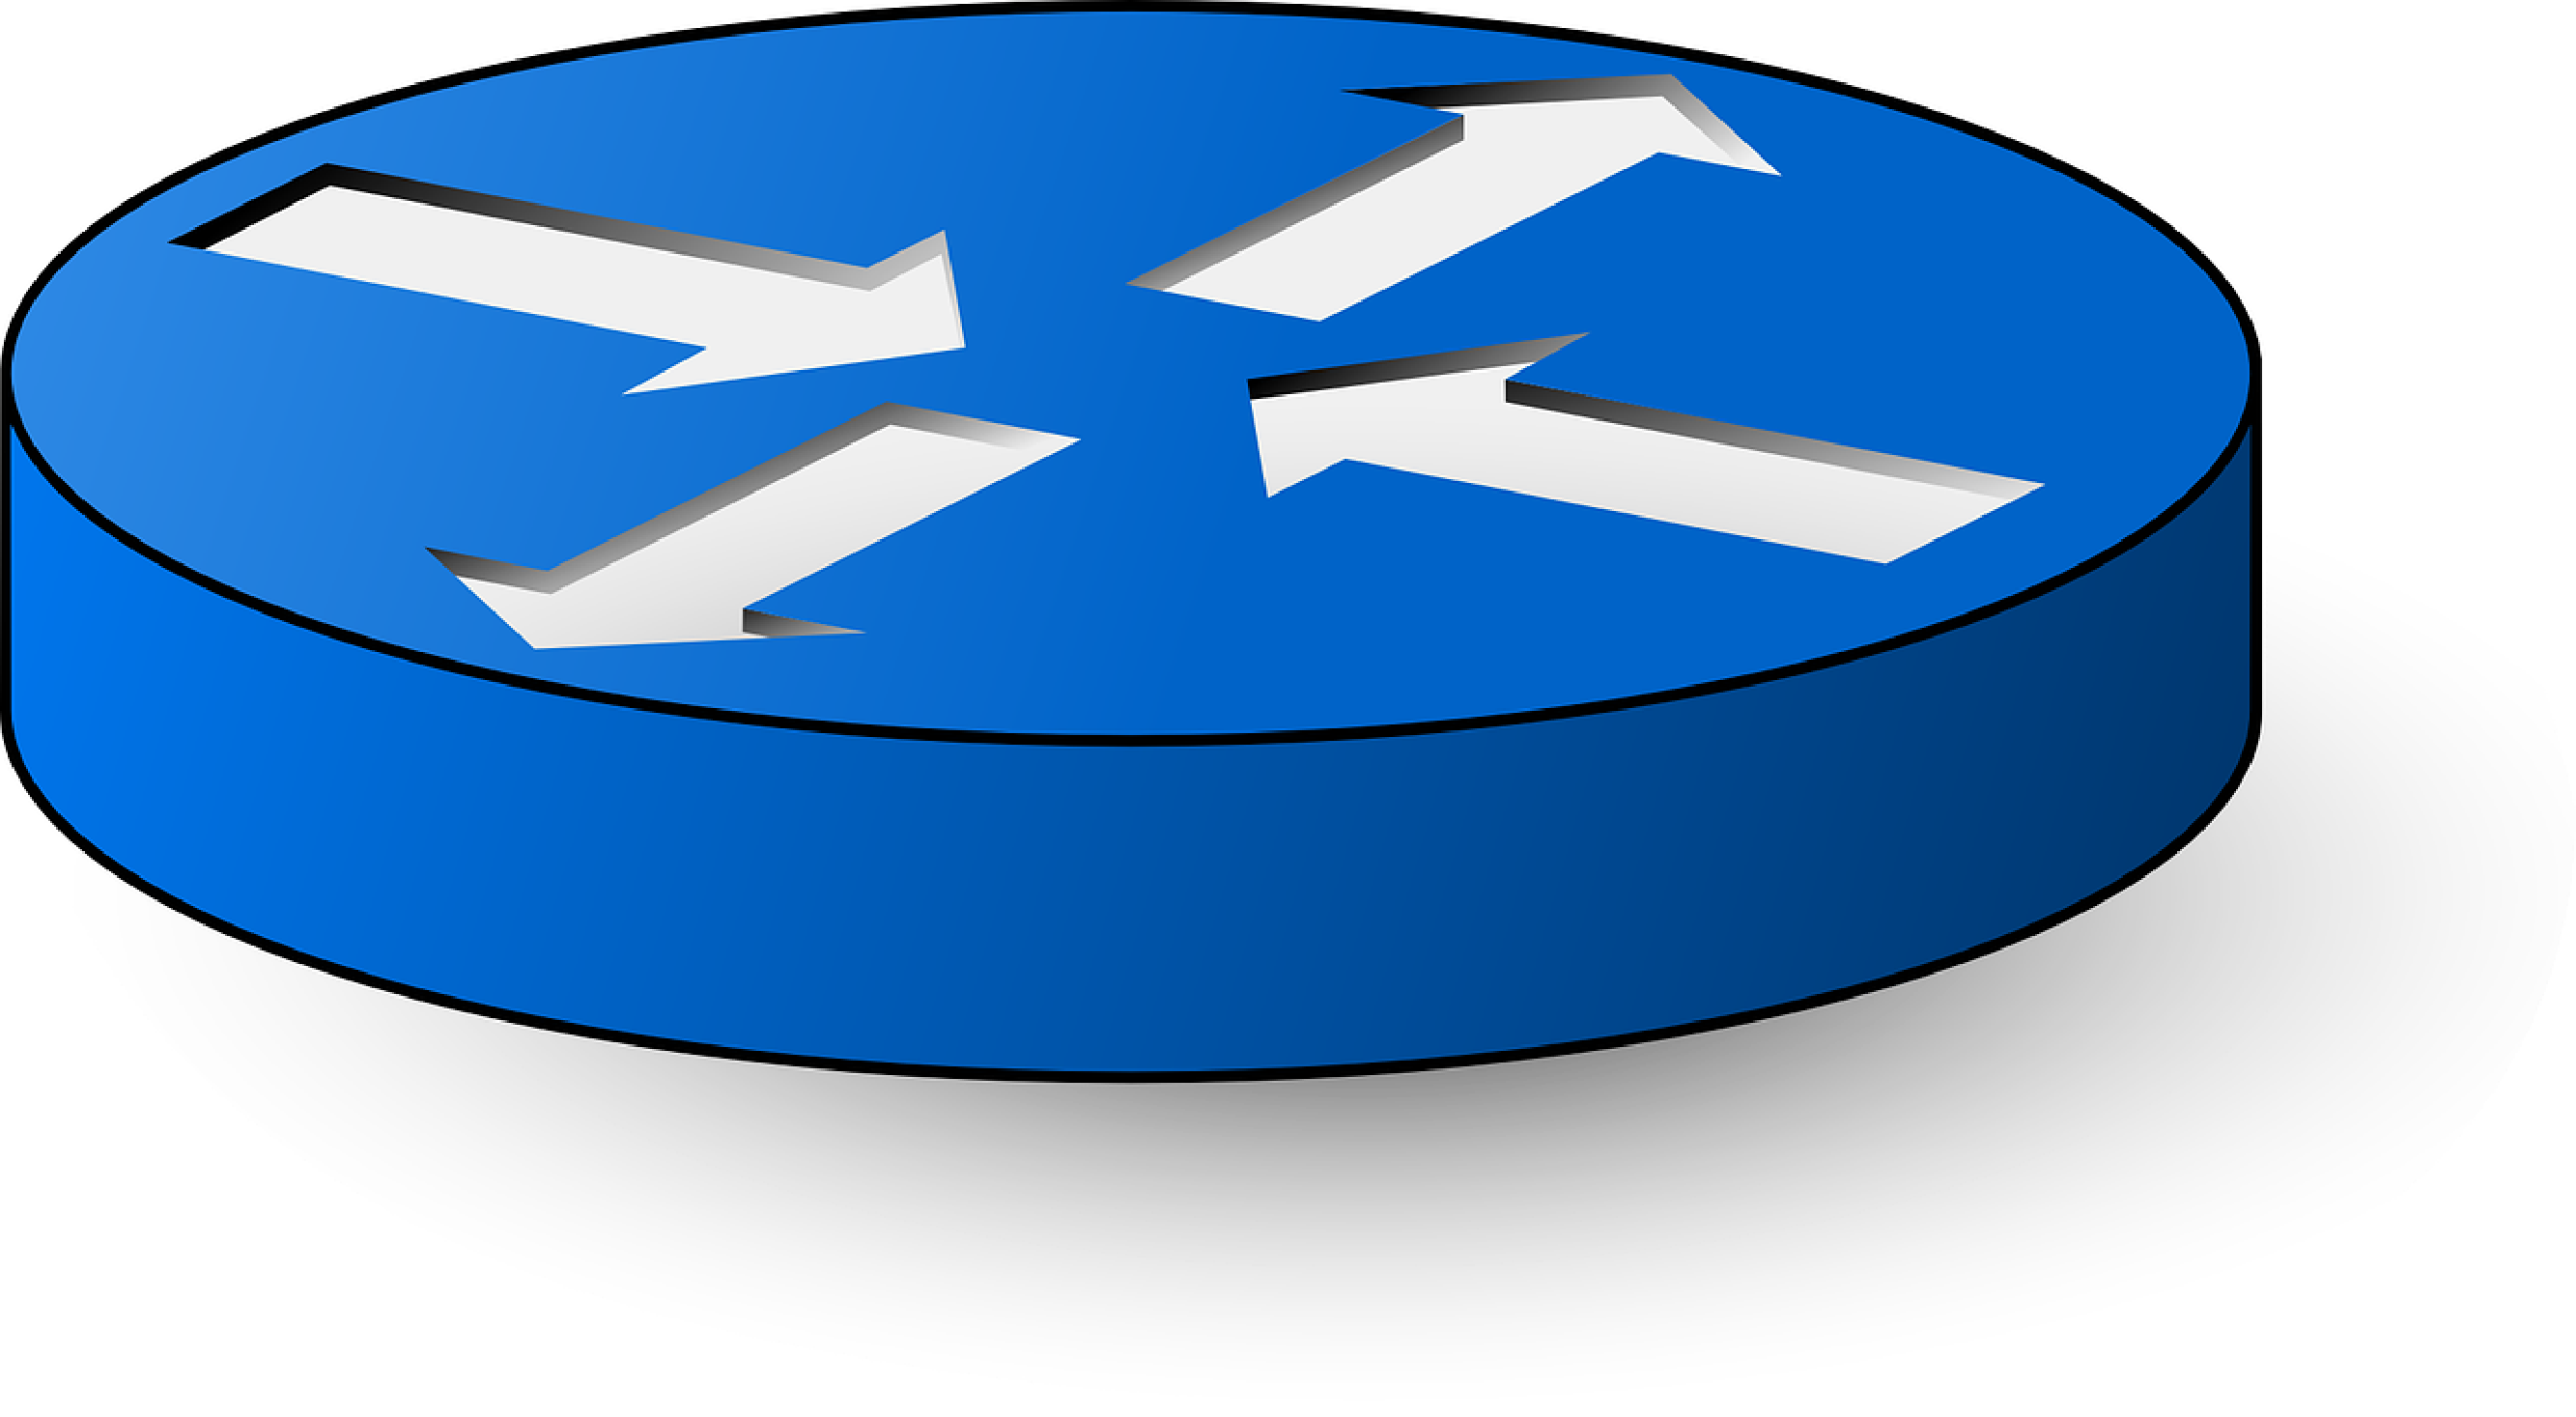
\includegraphics[width=52.5pt,height=52.5pt]{figures/router-30140_1280.pdf}};
%Image [id:dp34021892319279323] 
\draw (515,487.5) node  {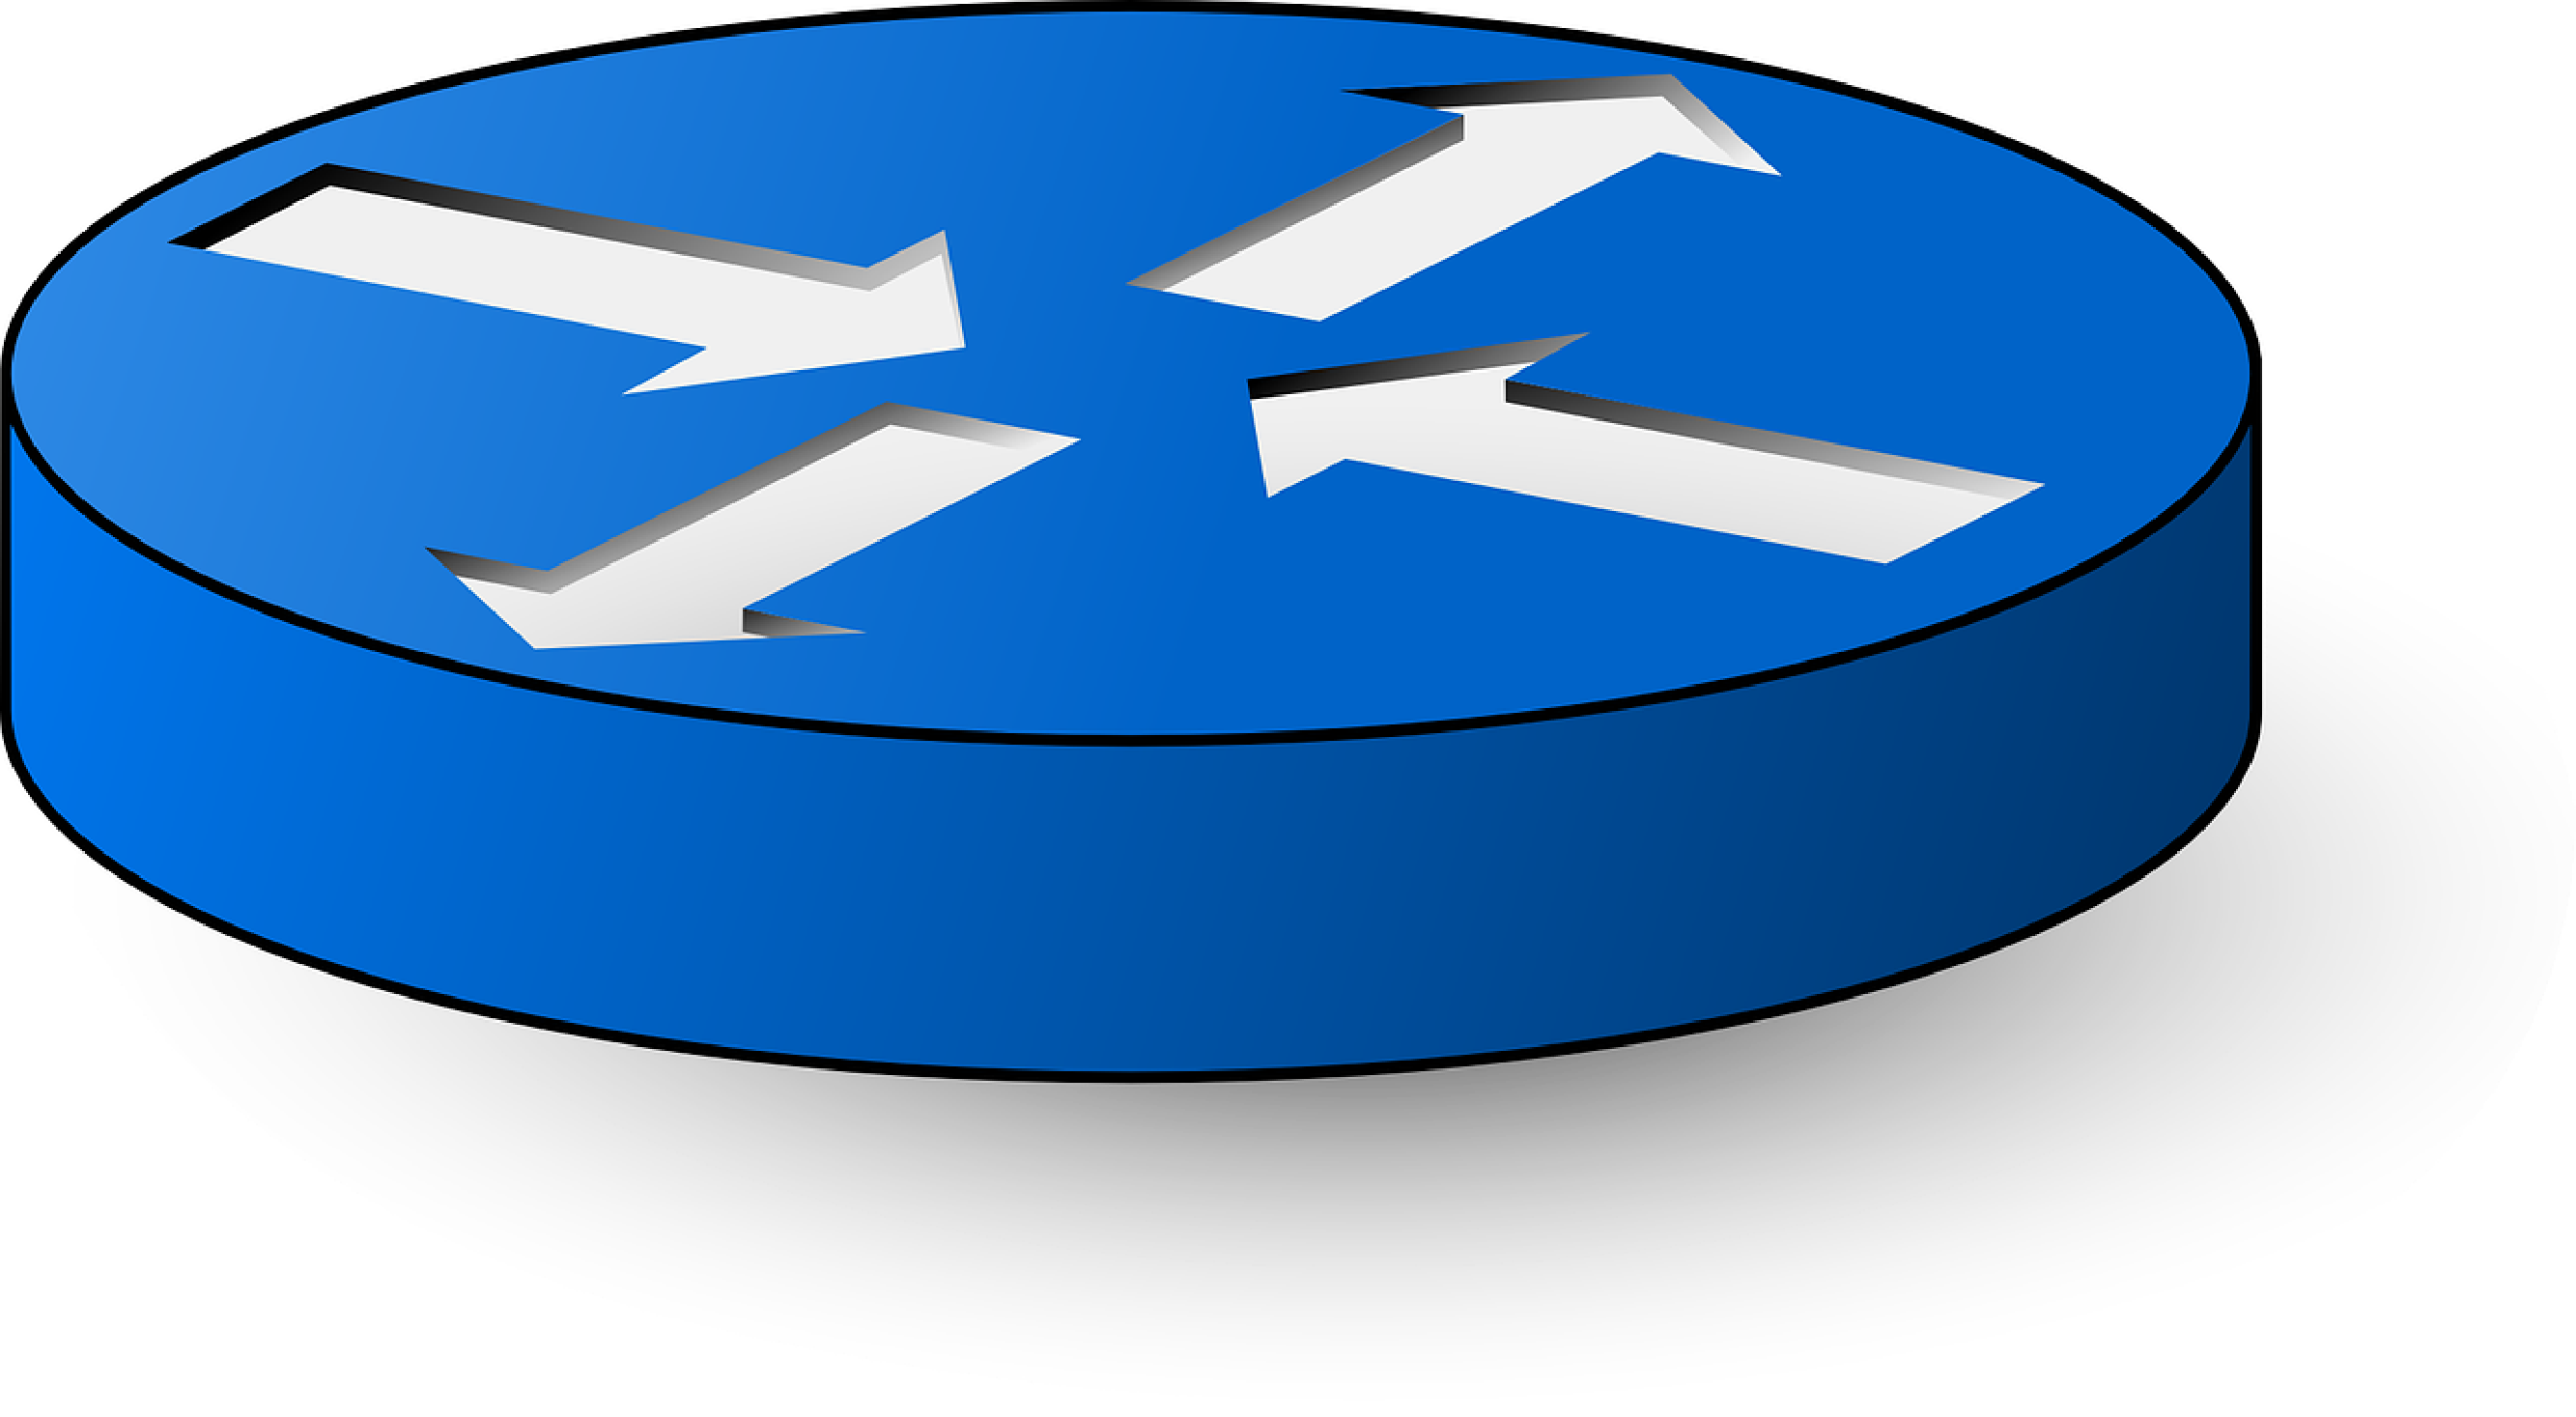
\includegraphics[width=52.5pt,height=52.5pt]{figures/router-30140_1280.pdf}};
%Straight Lines [id:da9221433559107663] 
\draw [line width=1.5]  [dash pattern={on 1.69pt off 2.76pt}]  (63.05,209) -- (62,408.97) ;


%Straight Lines [id:da18979728678812846] 
\draw [line width=1.5]  [dash pattern={on 1.69pt off 2.76pt}]  (139.05,261) -- (140,442.97) ;


%Straight Lines [id:da3949095016333407] 
\draw [line width=1.5]  [dash pattern={on 1.69pt off 2.76pt}]  (178.05,153) -- (186.2,381.27) ;


%Straight Lines [id:da9197957685386293] 
\draw [line width=1.5]  [dash pattern={on 1.69pt off 2.76pt}]  (314.05,169.17) -- (84,411) ;


%Straight Lines [id:da5299009760945013] 
\draw [line width=1.5]  [dash pattern={on 1.69pt off 2.76pt}]  (492.05,168) -- (495.6,384.07) ;


%Straight Lines [id:da535589916512549] 
\draw [line width=1.5]  [dash pattern={on 1.69pt off 2.76pt}]  (390.05,170) -- (390.4,391.27) ;


%Rounded Rect [id:dp33971726070681063] 
\draw  [fill={rgb, 255:red, 217; green, 154; blue, 232 }  ,fill opacity=1 ] (49,306.78) .. controls (49,301.88) and (52.98,297.9) .. (57.89,297.9) -- (543.11,297.9) .. controls (548.02,297.9) and (552,301.88) .. (552,306.78) -- (552,333.45) .. controls (552,338.35) and (548.02,342.33) .. (543.11,342.33) -- (57.89,342.33) .. controls (52.98,342.33) and (49,338.35) .. (49,333.45) -- cycle ;

%Straight Lines [id:da3032548642460361] 
\draw [color={rgb, 255:red, 74; green, 144; blue, 226 }  ,draw opacity=1 ][line width=1.5]    (222.05,340.17) -- (208.13,376.37) ;
\draw [shift={(207.05,379.17)}, rotate = 291.04] [color={rgb, 255:red, 74; green, 144; blue, 226 }  ,draw opacity=1 ][line width=1.5]    (14.21,-4.28) .. controls (9.04,-1.82) and (4.3,-0.39) .. (0,0) .. controls (4.3,0.39) and (9.04,1.82) .. (14.21,4.28)   ;

%Straight Lines [id:da5649833646600878] 
\draw [color={rgb, 255:red, 74; green, 144; blue, 226 }  ,draw opacity=1 ][line width=1.5]    (330.05,344.17) -- (369.08,388.91) ;
\draw [shift={(371.05,391.17)}, rotate = 228.9] [color={rgb, 255:red, 74; green, 144; blue, 226 }  ,draw opacity=1 ][line width=1.5]    (14.21,-4.28) .. controls (9.04,-1.82) and (4.3,-0.39) .. (0,0) .. controls (4.3,0.39) and (9.04,1.82) .. (14.21,4.28)   ;

%Straight Lines [id:da5842761266197537] 
\draw [color={rgb, 255:red, 74; green, 144; blue, 226 }  ,draw opacity=1 ][line width=1.5]    (479.05,343.17) -- (485.53,380.21) ;
\draw [shift={(486.05,383.17)}, rotate = 260.07] [color={rgb, 255:red, 74; green, 144; blue, 226 }  ,draw opacity=1 ][line width=1.5]    (14.21,-4.28) .. controls (9.04,-1.82) and (4.3,-0.39) .. (0,0) .. controls (4.3,0.39) and (9.04,1.82) .. (14.21,4.28)   ;

%Straight Lines [id:da44476437360701715] 
\draw [color={rgb, 255:red, 74; green, 144; blue, 226 }  ,draw opacity=1 ][line width=1.5]    (93.05,345.17) -- (75.9,403.29) ;
\draw [shift={(75.05,406.17)}, rotate = 286.44] [color={rgb, 255:red, 74; green, 144; blue, 226 }  ,draw opacity=1 ][line width=1.5]    (14.21,-4.28) .. controls (9.04,-1.82) and (4.3,-0.39) .. (0,0) .. controls (4.3,0.39) and (9.04,1.82) .. (14.21,4.28)   ;

%Straight Lines [id:da5384124591664345] 
\draw [line width=1.5]  [dash pattern={on 1.69pt off 2.76pt}]  (445.5,16.33) -- (484.5,16.83) ;


%Straight Lines [id:da3606010400838229] 
\draw    (445,32.71) -- (485,33.21) ;


%Straight Lines [id:da015844815365207543] 
\draw [color={rgb, 255:red, 74; green, 144; blue, 226 }  ,draw opacity=1 ][line width=1.5]    (448.5,65.13) -- (478.5,64.97) ;
\draw [shift={(481.5,64.96)}, rotate = 539.71] [color={rgb, 255:red, 74; green, 144; blue, 226 }  ,draw opacity=1 ][line width=1.5]    (14.21,-4.28) .. controls (9.04,-1.82) and (4.3,-0.39) .. (0,0) .. controls (4.3,0.39) and (9.04,1.82) .. (14.21,4.28)   ;

%Straight Lines [id:da6059698523065559] 
\draw [color={rgb, 255:red, 74; green, 144; blue, 226 }  ,draw opacity=1 ][line width=1.5]    (161,343) -- (155.18,439.01) ;
\draw [shift={(155,442)}, rotate = 273.47] [color={rgb, 255:red, 74; green, 144; blue, 226 }  ,draw opacity=1 ][line width=1.5]    (14.21,-4.28) .. controls (9.04,-1.82) and (4.3,-0.39) .. (0,0) .. controls (4.3,0.39) and (9.04,1.82) .. (14.21,4.28)   ;

%Straight Lines [id:da7790467806562547] 
\draw [color={rgb, 255:red, 74; green, 144; blue, 226 }  ,draw opacity=1 ][line width=1.5]    (433,343) -- (487.71,458.29) ;
\draw [shift={(489,461)}, rotate = 244.61] [color={rgb, 255:red, 74; green, 144; blue, 226 }  ,draw opacity=1 ][line width=1.5]    (14.21,-4.28) .. controls (9.04,-1.82) and (4.3,-0.39) .. (0,0) .. controls (4.3,0.39) and (9.04,1.82) .. (14.21,4.28)   ;


% Text Node
\draw (85,498.5) node [scale=0.9] [align=left] {Physical Infrastructure};
% Text Node
\draw (59,137) node  [align=left] {V1};
% Text Node
\draw (119,117) node  [align=left] {V3};
% Text Node
\draw (144,188) node  [align=left] {V2};
% Text Node
\draw (353,111) node  [align=left] {V4};
% Text Node
\draw (437,113) node  [align=left] {V5};
% Text Node
\draw (512,108) node  [align=left] {V6};
% Text Node
\draw (54,475) node  [align=left] {P1};
% Text Node
\draw (205,486) node  [align=left] {P2};
% Text Node
\draw (244,390) node  [align=left] {P3};
% Text Node
\draw (342,397) node  [align=left] {P4};
% Text Node
\draw (561,394) node  [align=left] {P5};
% Text Node
\draw (565,473) node  [align=left] {P6};
% Text Node
\draw (531,16) node  [align=left] {Virtual Link};
% Text Node
\draw (538,37) node  [align=left] {Physical Link};
% Text Node
\draw (572,59) node  [align=left] {Hypervisor - Switch link};
% Text Node
\draw (300.5,320.11) node  [align=left] {Network Hypervisor : hname1};
% Text Node
\draw (69,104.5) node  [align=left] {{\small vSDN1}};
% Text Node
\draw (309,97.5) node [scale=0.9] [align=left] {{\small vSDN2}};


\end{tikzpicture}

\caption{Example of infrastructure  modeling}
\label{fig:VNE-example-model}
\end{figure}

The current infrastructure gives the following formal declaration:

\begin{lstlisting}[backgroundcolor = \color{lightgray}]
virtual_network(vSDN1,ti)
virtual_network(vSDN2,ti)
virtual_node(V1,vSDN1,ti)
virtual_node(V2,vSDN1,ti)
virtual_node(V3,vSDN1,ti)
virtual_node(V4,vSDN2,ti)
virtual_node(V5,vSDN2,ti)
virtual_node(V6,vSDN2,ti)
virtual_link(vlink1,V1,V2,vSDN1,ti)
virtual_link(vlink2,V1,V3,vSDN1,ti)
virtual_link(vlink3,V4,V5,vSDN2,ti)
virtual_link(vlink4,V5,V6,vSDN2,ti)
physical_node(P1,ti)
physical_node(P2,ti)
physical_node(P3,ti)
physical_node(P4,ti)
physical_node(P5,ti)
physical_node(P6,ti)
physical_link(plink1,P1,P2,ti)
physical_link(plink2,P1,P3,ti)
physical_link(plink3,P2,P4,ti)
physical_link(plink4,P3,P4,ti)
physical_link(plink5,P4,P5,ti)
physical_link(plink6,P4,P6,ti)
physical_path(ppath1,P1,P1,ti)
physical_path(ppath2,P2,P2,ti)
physical_path(ppath3,P3,P3,ti)
physical_path(ppath4,P4,P4,ti)
physical_path(ppath5,P5,P5,ti)
physical_path(ppath6,P6,P6,ti)
hypervisor(hyp1,ti)
hypervisor_of(hyp1,P1,ppath1,ti)
hypervisor_of(hyp1,P2,ppath2,ti)
hypervisor_of(hyp1,P3,ppath3,ti)
hypervisor_of(hyp1,P4,ppath4,ti)
hypervisor_of(hyp1,P5,ppath5,ti)
hypervisor_of(hyp1,P6,ppath6,ti)
node_embedding(V1,P1,ti)
node_embedding(V4,P1,ti)
node_embedding(V2,P2,ti)
node_embedding(V3,P3,ti)
node_embedding(V5,P4,ti)
node_embedding(V6,P5,ti)
link_embedding(vlink1,plink1,ti)
link_embedding(vlink2,plink2,ti)
link_embedding(vlink3,plink1,ti)
link_embedding(vlink3,plink4,ti)
link_embedding(vlink4,plink5,ti)
\end{lstlisting}